%%% %%% %%% %%%%%%%%%%%%%%%%%%%%%%%% %%% %%% %%%
%%% %%% %%% (1) Defintions And Stuff %%% %%% %%%
%%% %%% %%% %%%%%%%%%%%%%%%%%%%%%%%% %%% %%% %%%

		%%% %%%%%%%%%%%%%%%%%%%%%%%%%%%%%%%%%%%% %%%
		%%% Required Packages and Configurations %%%
		%%% %%%%%%%%%%%%%%%%%%%%%%%%%%%%%%%%%%%% %%%
		\RequirePackage{scrlfile}
		\IfFileExists{../common/hpibpthesis.cls}{
			\ReplaceFile{hpibpthesis.cls}{../common/hpibpthesis.cls}
		}{}
		
		\documentclass{hpibpthesis}
		\usepackage[htt]{hyphenat}
		% JavaScript syntax highlighting

\usepackage{color}
\usepackage[usenames,dvipsnames]{xcolor}

\colorlet{stringcolor}{red!60!black}
\definecolor{delim}{RGB}{20,105,176}

\lstdefinelanguage{JavaScript}{
    keywords={true, false, null},
    keywordstyle=\color{blue}\bfseries,
    identifierstyle=\color{black}\bfseries,
    sensitive=false,
    comment=[l]{//},
    morecomment=[s]{/*}{*/},
    commentstyle=\color{gray}\ttfamily,
    stringstyle=\color{stringcolor}\ttfamily\bfseries,
    morestring=[b]',
    morestring=[b]",
		showstringspaces=false,
		captionpos=b,
    literate=
       *{:}{{{\color{delim}\bfseries{:}}}}{1}
        {,}{{{\color{delim}\bfseries{,}}}}{1}
        {\{}{{{\color{delim}\bfseries{\{}}}}{1}
        {\}}{{{\color{delim}\bfseries{\}}}}}{1}
        {[}{{{\color{delim}\bfseries{[}}}}{1}
        {]}{{{\color{delim}\bfseries{]}}}}{1},
}
		\setcounter{secnumdepth}{2}

		%%% %%%%%%%%%%%%%%%%%%%%%%%%%% %%%
		%%% Define Document Properties %%%
		%%% %%%%%%%%%%%%%%%%%%%%%%%%%% %%%
		\title{Historische Betriebssysteme für InstantLab}
		\othertitle{Historic Operating Systems for InstantLab}
		\author{Felix Jankowski}
		\date{31. März 2014}
		\tenderdate{31. März 2014}
		\subject{Betriebssysteme und Middleware}
		\place{Potsdam}
		\professor{Prof. Dr. Polze}
		\supervisors{Dipl-Inf. Christian Neuhaus}
		\organisation{Hasso-Plattner-Institut an der Universität Potsdam}

		%%% %%%%%%%%%%%%%%%%%%%%% %%%
		%%% Define Chapter States %%%
		%%% %%%%%%%%%%%%%%%%%%%%% %%%
		%\definecontentblockstate{plan}{false}{0.5,0.5,0.5}{2cm}
		%\definecontentblockstate{question}{false}{0.0,0.0,1.0}{2cm}
		%\definecontentblockstate{research}{false}{1.0,0.0,0.0}{2cm}
		%\definecontentblockstate{draft}{false}{0.0,0.6,0.1}{0cm}
		%\definecontentblockstate{finish}{true}{0.0,0.6,0.1}{2cm}
		%\definecontentblockstate{work}{false}{0.0,0.0,1.0}{2cm}

		%%% %%%%%%%%%%%%%%%% %%%
		%%% Define Shortcuts %%%
		%%% %%%%%%%%%%%%%%%% %%%		
		\newcommand{\todo}[1]{
			\colorbox{black}{
				\textcolor{white}{
					\large{ TODO: #1 }
				}
			}
		}
		\newcommand{\note}[1]{
			\colorbox{black}{
				\textcolor{white}{
					#1
				}
			}
		}
		\newcommand{\question}[1]{
			\colorbox{red}{
				\textcolor{white}{
					FRAGE: #1
				}
			}
		}
		\newcommand{\idea}[1]{
			\colorbox{blue}{
				\textcolor{white}{
					IDEE: #1
				} 
			}
		}
		
		%%% %%%%%%%%%%%%%%%%%% %%%
		%%% Load Glossary Data %%%
		%%% %%%%%%%%%%%%%%%%%% %%%
		\nocite{*}

		\makeglossaries
		\loadglsentries{extra/glossary}
		%\bibliography{../common/bp2012m2}
		\bibliography{extra/literatur}



%%% %%% %%% %%%%%%%%%%%%%%%%% %%% %%% %%%
%%% %%% %%% (2) Main Document %%% %%% %%%
%%% %%% %%% %%%%%%%%%%%%%%%%% %%% %%% %%%
\begin{document}

		%%% %%%%%%%%%%%%%%%%%%%%%%%%%%%%%%%%%%%%%%%%%%%%%% %%%
		%%% Load Initial Stuff (Titlepage, Contents, ...)  %%%
		%%% %%%%%%%%%%%%%%%%%%%%%%%%%%%%%%%%%%%%%%%%%%%%%% %%%
		\maketitle[0]
		\singlespace
		\begin{abstract}

		\section*{Kurzdarstellung}

		Die historische Entwicklung der Betriebssysteme bis hin zum heutigen Windows 8.1 ist ein wichtiger Teil einer jeden ''Operating Systems''-Lehrveranstaltung an Universitäten.
		Während fast alle Themen im Informatikstudium mit praktischen Übungen vertieft werden, wird dies meist lediglich theoretisch als historische Abhandlung vermittelt.

		In dieser Arbeit wird eine Sammlung von verschiedenen Microsoft-Betriebssystemen in Form von virtuellen Maschinen zusammengestellt.
		Mit eigens entwickelten, didaktischen Experimenten können den Studenten damit die einzelnen Entwicklungsstufen der Betriebssysteme mit ihren Innovationen näher gebracht werden.
		Für die einfache Verwendung beinhalten die virtuellen Maschinen alle notwendigen Treiber und können in die InstantLab-Plattform des Lehrstuhls für Betriebssysteme und Middleware integriert werden.

\end{abstract}

		\tableofcontents

		%%% %%%%%%%%%%%%%%%%%%%%%%%%%% %%%
		%%% Load Main Document Content %%%
		%%% %%%%%%%%%%%%%%%%%%%%%%%%%% %%%
		%%% %%%%%%%%%%%%%%%%%%%%%%%%%%%%%% %%%
%%% Main Chapter 1 : Introduction  %%%
%%% %%%%%%%%%%%%%%%%%%%%%%%%%%%%%% %%%
\chapter{Einleitung}
\label{chap:introduction}


%%%%%%%%%%%%%%%%%%%%%%%%%%%%%%%%%%%%%%%%%%%%%%%%%%%%%%%%%%%%%%%%%%%%%%%%%%%%%%%%%%%%%%%%%%%%%%%%%%%%%%%%%
%\section{Über die Evolution der Betriebsysteme}
%\label{sec:evolution}
\section{Betriebsystemlehrveranstaltungen im Grundstudium}
\label{sec:motivation}
%%%%%%%%%%%%%%%%%%%%%%%%%%%%%%%%%%%%%%%%%%%%%%%%%%%%%%%%%%%%%%%%%%%%%%%%%%%%%%%%%%%%%%%%%%%%%%%%%%%%%%%%%

		Seit der Einrichtung des Studiengangs Informatik um das Jahr 1970 in Deutschland haben sich die Studieninhalte, insbesondere im Bereich "`Praktische Informatik"', stark verändert.
		Dies ist auch nicht weiter verwunderlich, da wohl keine Wissenschaft einer derart schnellen Weiterentwicklung unterliegt.

		Beispielsweise wurde Ende der 70er Jahre durch Alan Kays neue Programmiersprache Smalltalk die Objektorientierung eingeführt und mit ihr die Paradigmen der Programmierung grundlegend verändert.
		Mitte der 80er wurde durch die Verbreitung von Patterns die Softwarearchitektur grundlegend vereinfacht und standardisiert.
		In den 90ern verbreiteten sich schließlich Netzwerktechnologien, auf die natürlich auch in der Lehre eingegangen werden musste.

		Nahezu als Konstante lässt sich jedoch feststellen, dass von Anbeginn bis Heute im Grundstudium bzw. Bachelor eine Vorlesung zum Thema Betriebssysteme zwingend vorgeschrieben ist.
		Dabei stellt sich bei vielen Studenten die Frage, warum trotz der zahlreichen modernen Abstraktionsschichten (e.g. VMs bei Java und .net) einer grundlegenden und hardwarenahem Veranstaltung nach wie vor eine derartige Wichtigkeit eingeräumt wird.
		% Meist wird vorgeschlagen, eine derartige Veranstaltung als Wahl im Master für Interesse Treiber / Betriebssystem

		%Ressourcen
		%Sicherheit
		%Überlast

		Diese Frage lässt sich recht gut beantworten, wenn man beispielsweise das Verhalten von Rechnern unter Ressourcenknappheit betrachtet.
		Hierbei existieren zahlreiche, auch für Anwendungsprogrammierer relevante Probleme, deren Lösung nur mit Fachwissen über die internen Mechanismen des verwendeten Betriebssystems möglich ist. 
		Beispielsweise entstehen ohne Kenntnisse über Scheduling leicht Fehler im Bereich der Nebenläufigkeit, die nicht selten Programme durch Dead-Locks unbenutzbar machen und durch die Beeinflussung des Systems durch einen Debugger enorm schwer zu beheben sind (Heisenbugs).


		% Single User Single Task to Multi User Multi Task Scheduler beobachten, etc.

		% 		Von DOS 1.0 zu Windows 8


%%%%%%%%%%%%%%%%%%%%%%%%%%%%%%%%%%%%%%%%%%%%%%%%%%%%%%%%%%%%%%%%%%%%%%%%%%%%%%%%%%%%%%%%%%%%%%%%%%%%%%%%%
\section{Behandlung in der Lehre}
\label{sec:teaching}
%%%%%%%%%%%%%%%%%%%%%%%%%%%%%%%%%%%%%%%%%%%%%%%%%%%%%%%%%%%%%%%%%%%%%%%%%%%%%%%%%%%%%%%%%%%%%%%%%%%%%%%%%

		Eine gute Möglichkeit die verschiedenen Funktionen eines heutigen Betriebssystems kennen zu lernen besteht darin, dessen Evolution nachzuvollziehen. Hierbei wird nicht nur die Funktionsweise, sondern auch die Notwendigkeit jedes Features deutlich. 
		Bekanntermaßen führt unter Windows 3.11 eine Endlosschleife zum Absturz des gesamten Systems, da beim kooperativen Multitasking die CPU nicht mehr freigegeben wird.
		Um dieses extrem häufige Ärgernis zu beseitigen wurde mit Windows 95 (teilweise) präemptives Multitasking eingeführt.

		In Vorlesungen wird dies meistens behandelt, indem  die Entwicklung anhand historischer Daten vorgetragen wird.
		Das Lernen von Fakten und Versionsnummern bzw. Jahreszahlen führt meist jedoch nicht zum gleichen Verständnis wie das selbstständige Nachvollziehen von Problemen und deren Lösungen.
		Die anderen Themen der Lehrveranstaltung werden daher meist mittels praktischer Experimente vertieft.
		Bei diesen lösen Studenten selbstständig oder in Gruppen bestimmte Aufgaben und erleben daher die Funktionalitäten praxisnah.
		Bislang werden diese meist auf dem eigenen Computer oder in bereitgestellten virtuellen Maschinen gelöst.
		Hierbei kommt es immer wieder zu Problemen durch die notwendige Einrichtung und verschiedenartige Konfigurationen.

		Ein besonders innovatives Verfahren zur praxisnahen Lehre wird hierbei vom Hasso-Plattner-Institut angewendet.
		Beim OpenStack basierten InstantLab ist es für Studenten nicht mehr notwendig, die Experimente auf eigener Hardware einzurichten und durchzuführen.
		Stattdessen wird ein http-basiertes Interface angeboten, auf dem die Studenten nach einem Login mit ihrer Benutzerkennung (die Authentifikation erfolgt hierbei über den zentralen LDAP-Server des Instituts) auf Knopfdruck neue Instanzen eines VM-Templates erzeugen können. 
		Diese Templates werden vorher vom Übungsleiter bei der Aufgabenstellung angelegt und enthalten jeweils die Konfiguration einer VM sowie ein Datenträgerimage mit installiertem Betriebssystem und den für das jeweilige Experiment notwendigen Dateien.
		Die Experimente können ebenfalls vollständig im Webbrowser durchgeführt werden, dabei kommt eine Javascript basierte VNC Implementierung zum Einsatz.
		Die VMs können dort am Ende gespeichert und zur Benotung eingereicht werden.
		Sollten es im Laufe der Durchführung zu Problemen oder Fehlern kommen, kann die Instanz jederzeit gelöscht und neu aufgesetzt werden.

%%%%%%%%%%%%%%%%%%%%%%%%%%%%%%%%%%%%%%%%%%%%%%%%%%%%%%%%%%%%%%%%%%%%%%%%%%%%%%%%%%%%%%%%%%%%%%%%%%%%%%%%%
\section{Thema der Arbeit}
\label{sec:topic}
%%%%%%%%%%%%%%%%%%%%%%%%%%%%%%%%%%%%%%%%%%%%%%%%%%%%%%%%%%%%%%%%%%%%%%%%%%%%%%%%%%%%%%%%%%%%%%%%%%%%%%%%%
			


		%In dieser Arbeit sollen historische Betriebssysteme wieder ausführbar und erlebbar gemacht werden. 
		Ziel dieser Arbeit ist es, historische Betriebssysteme heutzutage für Studenten ausführbar zu machen.
		Da die damals verwendete Hardware schwer bis unmöglich zu replizieren ist, kommen hierbei virtuelle Maschinen zum Einsatz.
		Außerdem sollen mittels für diese Arbeit entwickelten und in diesen VMs ausführbaren Experimenten die Killer Features und die Neuerungen, aber auch die Nachteile, der jeweiligen Betriebssysteme erlebbar gemacht werden.
		
		Eine besondere Schwierigkeit liegt dabei darin begründet, dass die relevanten Systeme aufgrund ihres Alters längst das Ende des Supportzeitraums erreicht haben und auch von den Herstellern der Hypervisoren nicht mehr unterstützt werden oder noch nie unterstützt wurden.
		Daher existieren meist keine offiziellen Client-Treiber, dadurch ist insbesondere keine Paravirtualisierung möglich.
		Zudem ist die heutzutage virtualisierte Hardware meist deutlich neuer als diejenige, mit denen die Systeme ursprünglich auf Kompatibilität getestet wurden.

		Der Fokus liegt hierbei ausschließlich auf Betriebssystemen von Microsoft, da diese für heutige Programmierer die relevanteste Plattform darstellen.
		Zudem wurde hierbei stets auf Kompatibilität mit den Vorgängerversionen geachtet;
		insbesondere wurden allzu starke Veränderungen und komplette Neuentwicklungen größtenteils vermieden. 
		Daher lässt sich auf dieser Plattform die evolutionäre Weiterentwicklung der Software besonders gut beobachten. \\ \\

	
		%Desweiteren wurden von Microsoft alle Betriebssysteme für die Intel x86-Plattform angeboten, so dass auf Veränderungen des Systems durch unterschiedliche Hardware nicht geachtet werden muss.
		%Dass zwischenzeitlich auch andere Prozessoren, wie z.B. Itanium, von Windows NT unterstützt wurden, ist hierbei nicht von Relevanz. 

		%Gezielt Microsoft, historische Betriebssysteme und Killer-Features. 
				
		%Struktur

		Im Kapitel \ref{chap:challenges} (\nameref{chap:challenges}) werden die wichtigsten Ziele und Anforderungen erfasst. 
		Der Rest von Kapitel \ref{chap:challenges} ist der Recherche gewidmet; sowohl bestehende Lösungen als auch aktuelle akademische Diskussionen werden betrachtet.
		
		Das Hauptkapitel \ref{chap:setup} (\nameref{chap:setup}) dokumentiert die Erzeugung der Experimente von der Beschaffung historischer Betriebssysteme, der Wiederinbetriebnahme inkl. Anpassung an moderne Architekturen mittels spezieller Treiber bis zur Auswahl didaktisch geeigneter Experimente.
		Dabei wird zuerst der gewählte Ansatz und danach die konkreten Schritte für jede virtuelle Maschine vorgestellt.
		
		Das darauf folgenden Kapitel \ref{chap:experiments} (\nameref{chap:experiments}) beschreibt die Durchführung der Versuche und die zu erwartenden Ergebnisse aus Sicht des Studenten. Es kann später als Experimentierhandbuch verwendet werden.

		Zuletzt wird in Kapitel \ref{chap:evaluation} (\nameref{chap:evaluation}) das Ergebnis der Arbeit zusammenfassend dargestellt und bewertet, wobei auch auf noch nicht umgesetzte Ideen und Möglichkeiten eingegangen wird.
		


		%%% %%%%%%%%%%%%%%%%%%%%%%%%%%%% %%%
%%% Main Chapter 2 : Challenges  %%%
%%% %%%%%%%%%%%%%%%%%%%%%%%%%%%% %%%
\chapter{Darstellung der Evolution historischer Betriebssysteme}
\label{chap:challenges}


Auf neue Features wird nicht im einzelnen Eingegangen und statt dessen auf den Wikipediartikel Geschichte von Windows verwiesen??


%%%%%%%%%%%%%%%%%%%%%%%%%%%%%%%%%%%%%%%%%%%%%%%%%%%%%%%%%%%%%%%%%%%%%%%%%%%%%%%%%%%%%%%%%%%%%%%%%%%%%%%%%
\section{Zielsetzung}
\label{sec:aims}
%%%%%%%%%%%%%%%%%%%%%%%%%%%%%%%%%%%%%%%%%%%%%%%%%%%%%%%%%%%%%%%%%%%%%%%%%%%%%%%%%%%%%%%%%%%%%%%%%%%%%%%%%

		Es soll eine ... entworfen und umgesetzt werden.
		Der vorgesehene Anwendungsfall ist


		Cloud-Umgebung für virtuelle Maschinen
		herausragende Merkmale studieren und vor allem erleben



%%%%%%%%%%%%%%%%%%%%%%%%%%%%%%%%%%%%%%%%%%%%%%%%%%%%%%%%%%%%%%%%%%%%%%%%%%%%%%%%%%%%%%%%%%%%%%%%%%%%%%%%%
\section{Anforderungen}
\label{sec:requirements}
%%%%%%%%%%%%%%%%%%%%%%%%%%%%%%%%%%%%%%%%%%%%%%%%%%%%%%%%%%%%%%%%%%%%%%%%%%%%%%%%%%%%%%%%%%%%%%%%%%%%%%%%%

		Aus den oben genannten Zielen ergeben sich

		Auf Didaktik wird verzichtet
				
		%%%%%%%%%%%%%%%%%%%%%%%%%%%%%%
		\subsection{Funktionale Anforderungen}
		%%%%%%%%%%%%%%%%%%%%%%%%%%%%%%

		Use Case Diagramm

		Experiment -> Pakete
		Kursleiter
		Administrator
				
		%%%%%%%%%%%%%%%%%%%%%%%%%%%%%%
		\subsection{Nicht-Funktionale Anforderungen}
		%%%%%%%%%%%%%%%%%%%%%%%%%%%%%%

		Isolation
		Tamper-Proof
		Acccount
		evtl. Bewertung

	

%%%%%%%%%%%%%%%%%%%%%%%%%%%%%%%%%%%%%%%%%%%%%%%%%%%%%%%%%%%%%%%%%%%%%%%%%%%%%%%%%%%%%%%%%%%%%%%%%%%%%%%%%
\section{Vergleichbare System}
\label{sec:solutions}
%%%%%%%%%%%%%%%%%%%%%%%%%%%%%%%%%%%%%%%%%%%%%%%%%%%%%%%%%%%%%%%%%%%%%%%%%%%%%%%%%%%%%%%%%%%%%%%%%%%%%%%%%
		
		\subsection{Audacity}
		\subsection{Coursera}

		Kein Wissen über User
		keine Live-Experimente wie Instantlab

		Aber: Aufgabenabgabesystem
		
		Neugikeit: Instanz auf Knopfdruck
		
%%%%%%%%%%%%%%%%%%%%%%%%%%%%%%%%%%%%%%%%%%%%%%%%%%%%%%%%%%%%%%%%%%%%%%%%%%%%%%%%%%%%%%%%%%%%%%%%%%%%%%%%%
\section{Technologien}
\label{sec:technologies}
%%%%%%%%%%%%%%%%%%%%%%%%%%%%%%%%%%%%%%%%%%%%%%%%%%%%%%%%%%%%%%%%%%%%%%%%%%%%%%%%%%%%%%%%%%%%%%%%%%%%%%%%%

		Allgemeines zur Plattform und zur Virtualisierung

		Plattform Intel x86 / Microsoft wegen der durchgängigen Unterstützung. \cite{PopekGoldberg}

		Spezialfälle: Binary rewriting, manche Operationen schneller in Softwre als in Hardware

		Warum ist Intel problematisch??

		Typ 1/2 Virtualisierung (hier ggf. nicht relevant)


		%%%%%%%%%%%%%%%%%%%%%%%%%%%%%%%%%%%%%%%%%%%%%%%%%%%%%%%%%%%%
		\subsection{VMWare}
		%%%%%%%%%%%%%%%%%%%%%%%%%%%%%%%%%%%%%%%%%%%%%%%%%%%%%%%%%%%%

		Relevanz: Feld eröffnet, große Menge Hardware

		%%%%%%%%%%%%%%%%%%%%%%%%%%%%%%%%%%%%%%%%%%%%%%%%%%%%%%%%%%%%
		\subsection{KVM}
		%%%%%%%%%%%%%%%%%%%%%%%%%%%%%%%%%%%%%%%%%%%%%%%%%%%%%%%%%%%%

		Relevanz: Standard reportoire, Open Source

		
		%%% %%%%%%%%%%%%%%%%%%%%%%%%%%%%%%%% %%%
%%% Main Chapter 4 : Implementation  %%%
%%% %%%%%%%%%%%%%%%%%%%%%%%%%%%%%%%% %%%
\chapter{Setup}
\label{chap:setup}

	In diesem Kapitel wird beschrieben, wie ausgewählte historische Betriebssysteme im Rahmen dieser Arbeit wieder lauffähig gemacht wurden. Als Hypervisor kam, sofern nicht anderweitig vermerkt, VMWare Fusion Professional Version 6.0.2 auf Mac OS 10.9.2 zum Einsatz. 
	Die VMs werden zusammen mit dieser Arbeit eingereicht.

%%%%%%%%%%%%%%%%%%%%%%%%%%%%%%%%%%%%%%%%%%%%%%%%%%%%%%%%%%%%%%%%%%%%%%%%%%%%%%%%%%%%%%%%%%%%%%%%%%%%%%%%%
\section{PC DOS 1.10}
%%%%%%%%%%%%%%%%%%%%%%%%%%%%%%%%%%%%%%%%%%%%%%%%%%%%%%%%%%%%%%%%%%%%%%%%%%%%%%%%%%%%%%%%%%%%%%%%%%%%%%%%%

	MS DOS 1.0 stellt das erste Betriebssystem von Microsoft für die 8086-CPU dar. Es entstand durch eine Portierung von Tim Patersons QDOS auf den IBM PC und wurde mit diesem unter dem Namen IBM PC DOS vertrieben. \cite{WinHistory}
	Beim hier verwendeten PC DOS 1.10 handelt es sich um eine fehlerbereinigte, im Juli '82 veröffentlichte Version, die technisch MS DOS 1.25 entspricht. 
	Dieses Betriebssystem stellt größtenteils einen Nachbau von CP/M dar und war, außer durch das Vorhandensein des Dateisystems \gls{FAT}, wenig innovativ.
	Da es jedoch die Grundlage für den Erfolg von Microsoft und somit für alle späteren Betriebssysteme bildet, wird es in dieser Arbeit behandelt.

	DOS unterstützt in der Version 1 noch keine Festplatten und kann lediglich 5,25" Disketten bis 160 KB adressieren. \cite{WinHistory}
	Unter anderem aufgrund dieser Einschränkungen kann dieses Betriebssystem nicht mit zeitgemäßen Hypervisoren ausgeführt werden, statt dessen muss ein vollwertiger CPU- bzw. PC-Emulator wie Bochs oder QEMU verwendet werden. 

	Im "`Endangered Software Archive"', welches unter der URL \url{http://www.mirrors.org/archived_software/www.techknight.com/esa/default.htm} verfügbar ist, befindet sich eine mit dem "`Disk Image Archiver"' erstellte Kopie der originalen PC DOS 1.10 Startdiskette. 
	Mit einem Hex-Editor lässt sich aus dem proprietären .dim-Format eine Datei mit dem Inhalt der Diskette erstellen und das Betriebssystem in Bochs booten.
	Dieser Prozess ist in \cite{PCMinistry} beschrieben:

	Der Bootsektor der Diskette entspricht noch nicht den gängingen Industriestandards.
	So fehlt der BIOS Parameter Block, der bei allen FAT (ab DOS 2.0) und NTFS Dateisystemen den Aufbau des Datenträgersbeschreibt und Informationen über das Dateisystem enthält. Im vorliegenden Image ist dieser Bereich (ab Offset 07h) freigelassen.
	Modernere Betriebssysteme können die Diskette daher nicht lesen und geben aus, der Datenträger sei nicht korrekt formattiert. 
	Zudem wird die "`Boot Sektor Signatur"' am Ende des ersten Sektors (55h bei Offset 1FEh und AAh bei Offset 1FFh), welche ein Medium als bootbar markiert, vom BIOS bei Start noch nicht überprüft. \cite{IBMTechRef} Daher fehlt auch diese auf der Diskette und in dem Image sind am Ende des Bootsektors lediglich Nullen zu finden.
	Daher verweigert der Emulator den Bootvorgang.
	Ändert man mit einem Hex-Editor die Datei und schreibt 55AA an das Ende des Bootsektors, übergibt das BIOS die Kontrolle mittels JMP-Befehl an den in dem Image liegenden Code. Leider stürzt das System dann beim Bootvorgang ab.

	\begin{figure}[h]
		\begin{center}
			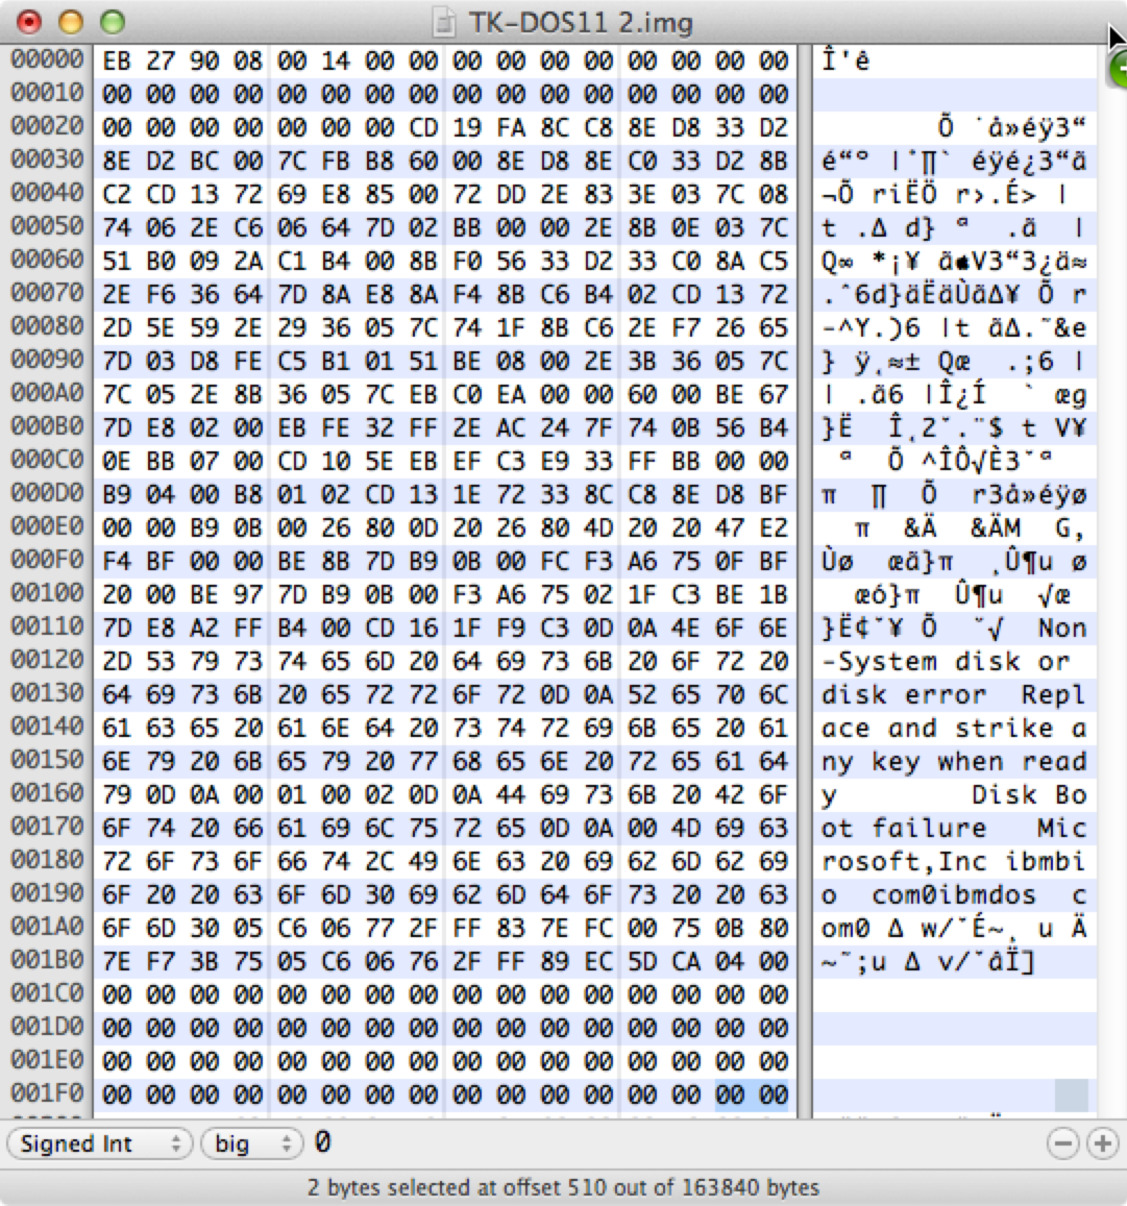
\includegraphics[width=0.7\textwidth]{img/DOS110hex}
			\caption{Ansicht des PC DOS 1.10 Bootsektors im Hex-Editor}
			\label{fig:screenshot-hexeditor110}
		\end{center}
	\end{figure}

	Glücklicherweise bietet Bochs bietet jedoch die Möglichkeit, die Überprüfung der Signatur zu deaktivieren und jeglichen Programmcode sofort zu booten, indem man \lstinline{floppy_bootsig_check: disabled=1} in das config file schreibt.
	Ein funktionierendes config File wird unter dem Namen $bochs.txt$ mit dieser Arbeit ausgeliefert.
	Hiermit lässt sich ein unverändertes Image von PC DOS 1.10 ausführen.
	Hierzu muss bochs im entsprechenden Verzeichnis gestartet werden, die Option \lstinline{2. Read options from ...} gewählt werden, mittels \lstinline{6. Begin simulation} der Emulator geladen werden und mit dem Befehl $continue$ die CPU gestartet werden.

	\begin{figure}[p]
		\begin{center}
			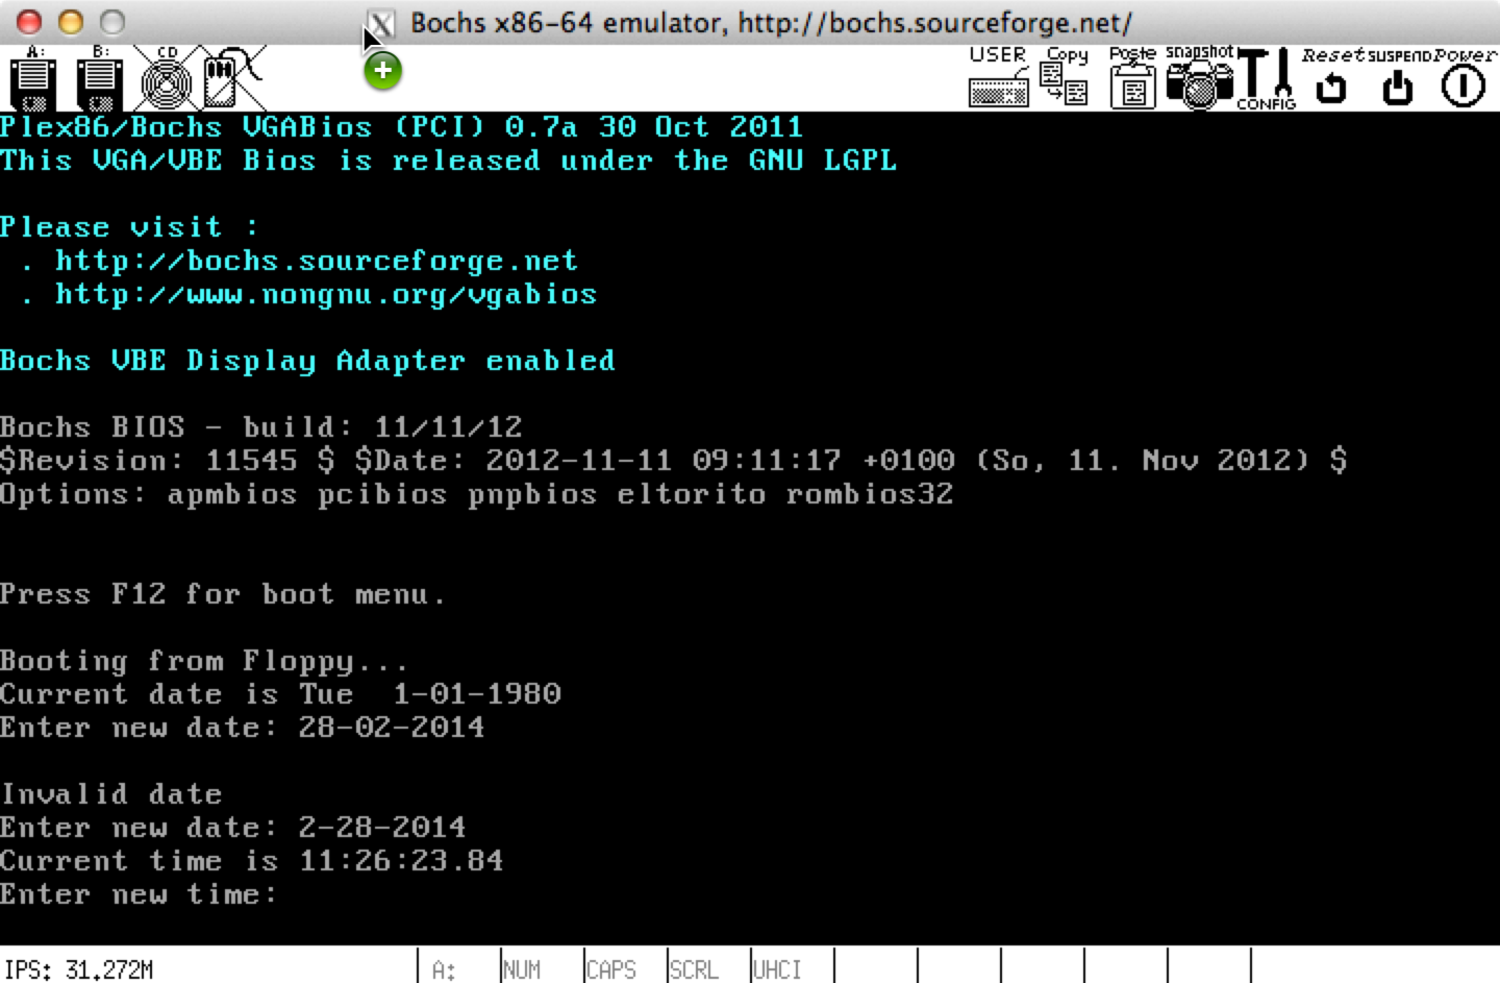
\includegraphics[width=\textwidth]{img/DOS110_1}
			\caption{Bootscreen von DOS 1.10}
			\label{fig:screenshot-dos110boot}
		\end{center}
	\end{figure}

	\begin{figure}[p]
		\begin{center}
			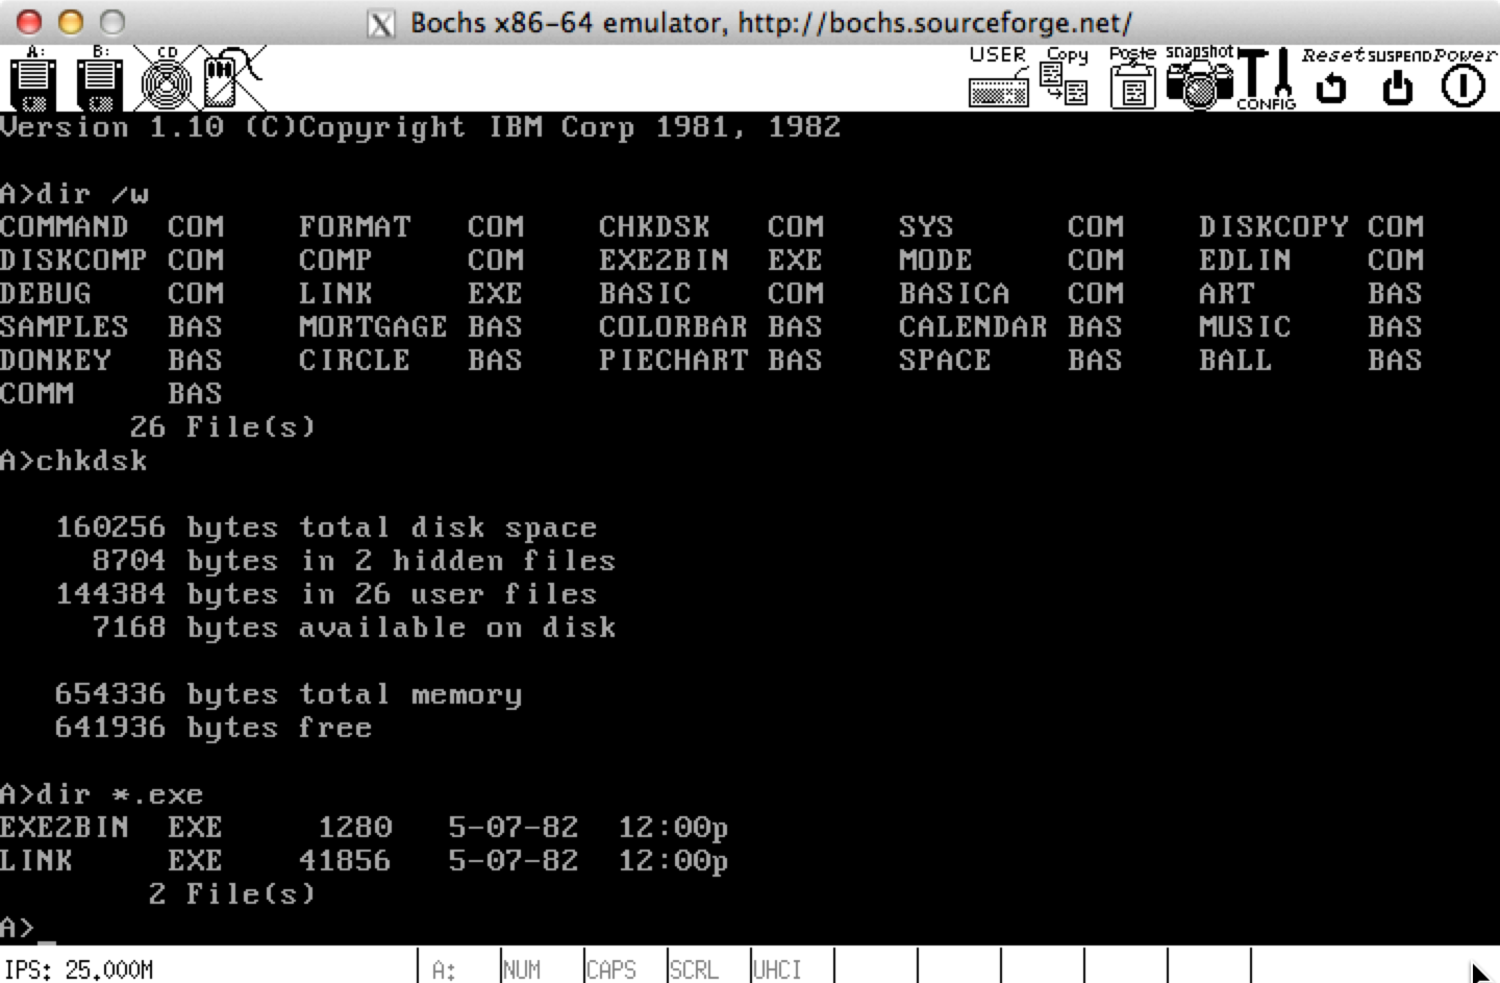
\includegraphics[width=\textwidth]{img/DOS110_2}
			\caption{Kommandos in PC DOS 1.10}
			\label{fig:screenshot-dos110commands}
		\end{center}
	\end{figure}

	Leider sind auch hier bei weitem nicht alle Funktionen des Betriebssystems benutzbar, da MS DOS sämtliche I/O-Operationen über die BIOS-Routinen durchführt.
	Das im originalen IBM PC verwendete BIOS unterscheidet sich jedoch signifikant von der "`BIOS Boot Specification"' vom 11. Januar 1996 und ist daher mit dem verwendeten Plex86/Bochs VGABios nicht kompatibel.

\newpage

%%%%%%%%%%%%%%%%%%%%%%%%%%%%%%%%%%%%%%%%%%%%%%%%%%%%%%%%%%%%%%%%%%%%%%%%%%%%%%%%%%%%%%%%%%%%%%%%%%%%%%%%%
\section{DOS 5.0 \& Windows 2.11}
%%%%%%%%%%%%%%%%%%%%%%%%%%%%%%%%%%%%%%%%%%%%%%%%%%%%%%%%%%%%%%%%%%%%%%%%%%%%%%%%%%%%%%%%%%%%%%%%%%%%%%%%%

	MS DOS 5.0 erschien im im Juni 1991.
	In den 10 Jahren seit der Veröffentlichung von PC-DOS 1.0 hatten sich zahlreiche Veränderungen ergeben. 
	Das Betriebssystem konnte nun auf Festplatten installiert werden, unterstütze 3,5''-Diskettenlaufwerke mit 720 KB, kannte Verzeichnisse in FAT, und konnte mittels Expanded Memory Specificatgion Arbeitsspeicher von mehr als 1 MB adressieren. 

	Windows 2.11 stellte einen Meilenstein dar, da es das erste Microsoft-Betriebssystem war das den protected mode des 386er Prozessors benutzte. Zudem bot es VGA-Unterstützung und neben kooperativem Multitasking auch die Möglichkeit, Fenster überlappen zu lassen.

	\begin{figure}[h]
		\begin{center}
			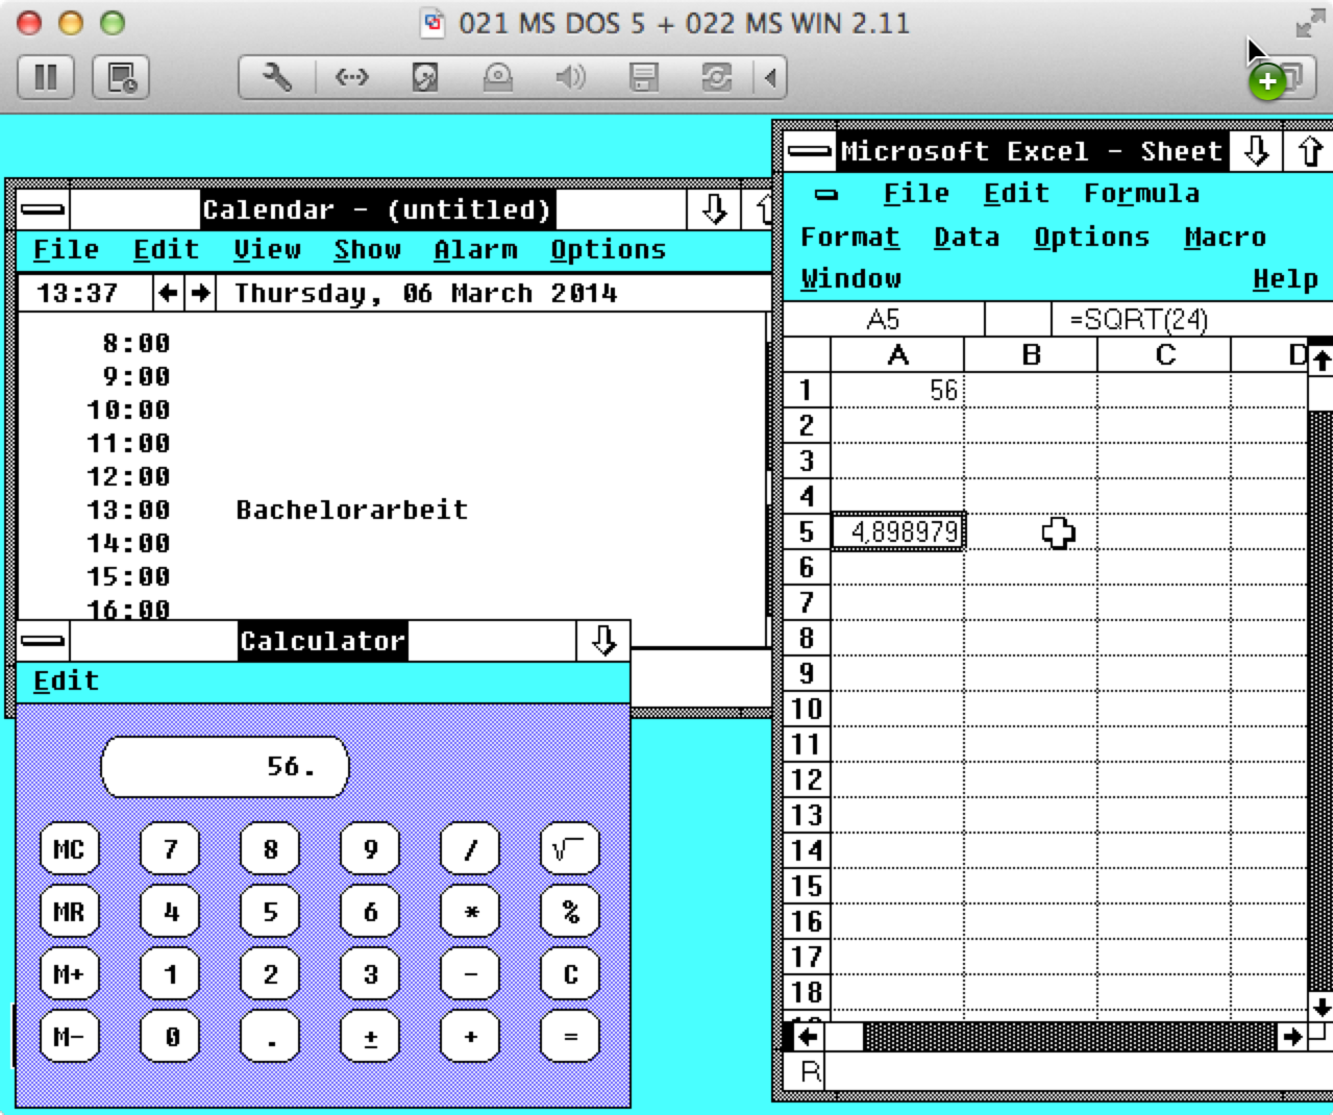
\includegraphics[width=\textwidth]{img/WIN211_2}
			\caption{Windows 2.11 mit Excel und einigen Standardprogrammen}
			\label{fig:screenshot-win211excel}
		\end{center}
	\end{figure}

	Im Rahmen dieser Arbeit wurden DOS 5.0 und Windows 2.11 auf 3,5''-Disketten gebraucht erworben und zudem ein USB-Floppylaufwerk bezogen.
	Leider gelang es nicht, diese originalen Disketten mit je 720 KB ("`Double Density"') auszulesen, da alle heutigen Betriebssysteme nur noch das Ansprechen von 1,44 MB-Datenträgern ("`High Density"') beherrschen.
	Versuche, den Inhalt der Disketten auszulesen schlagen daher mit der Meldung $I/O-Error$ fehl.
	Mit einem zufällig bei Autor noch vorhandenen Rechner mit Windows 95 war es ebenfalls nicht möglich die Daten auszulesen, da das integrierte Diskettenlaufwerk durch Alterung nicht mehr funktionierte.

	Images von beiden Systemen sind jedoch bei WinWorld\footnote{\url{http://wdl2.winworldpc.com/Abandonware\%20Operating\%20Systems/PC/DOS/Microsoft/}}, einem selbsternannten Online-Museum für Software verfügbar.
	Diese Images können in einer virtuellen Maschine als Diskettenlaufwerk gebootet werden, wenn als Betriebssystem MS-DOS konfiguriert und eine IDE-Festplatte mit weniger als 32 MB angelegt wird.
	Die Installation und der Betrieb von MS-DOS funktoinieren problemlos, allerdings kann nur RAM bis 1 MB adressiert werden.
	Dies gestaltet den Betrieb von Windows 2.11 kompliziert, aber nicht unmöglich.
	Bei der Installation muss explizit ausgewählt werden, Windows ohne extended memory installieren zu wollen, dann gelingt der Start.

	Einer der Hauptgründe für den Betrieb von Windows in der Version 2 war die Notwendigkeit, Excel ausführen zu müssen.
	Excel bringt eine eingeschränkte Windows-Runtime mit, damit es auch ohne eine Lizenz für Windows auf DOS-Rechnern ausgeführt werden kann.
	Es läuft jedoch besser unter einer Vollversion von Windows. 
	Zudem lassen sich damit bspw. Kalendereinträge übernehmen und Daten aus anderen Prozessen  kopieren.
	Aufgrund des historischen Kontexts, wird mit dieser VM eine Installation von Excel 2.1d mitgeliefert.

	Bei der Installation von Excel fällt auf, dass es in den gleichen Ordner wie Windows installiert werden muss (i.d.R. $C:\backslash{}Windows$). Zudem bringt es ein Programm namens $MemSet$ mit, welches den erweiterten Arbeitsspeicher konfiguriert und neue RAM-Treiber installiert. Mit diesem gelingt auch die Benutzung von RAM jenenseits der 1 MB.



	\begin{figure}[h]
		\begin{center}
			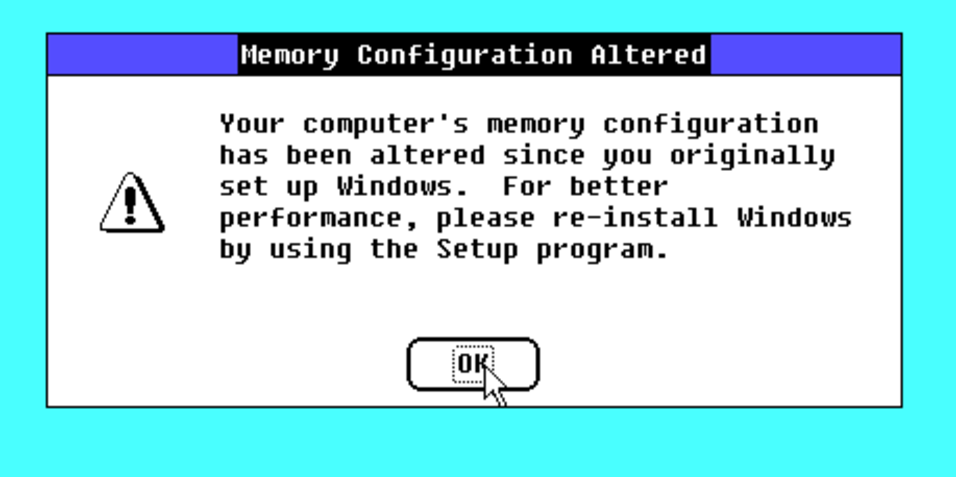
\includegraphics[width=0.7\textwidth]{img/WIN211_1}
			\caption{Warnung beim Start von Windows 2.11 nach der Installation von Excel}
			\label{fig:screenshot-win211error}
		\end{center}
	\end{figure}

\newpage

%%%%%%%%%%%%%%%%%%%%%%%%%%%%%%%%%%%%%%%%%%%%%%%%%%%%%%%%%%%%%%%%%%%%%%%%%%%%%%%%%%%%%%%%%%%%%%%%%%%%%%%%%
\section{DOS 6.0 \& Windows 3.11}
%%%%%%%%%%%%%%%%%%%%%%%%%%%%%%%%%%%%%%%%%%%%%%%%%%%%%%%%%%%%%%%%%%%%%%%%%%%%%%%%%%%%%%%%%%%%%%%%%%%%%%%%%
	Windows der dritten Generation war die erste auch bei Privatanwendern beliebte und kommerziell erfolgreiche Version des graphischen Betriebssystems von Microsoft.
	Zusätzlich wurde bei Version 3.11 Netzwerkfunktionalität eingeführt.

	Aus der gleichen Zeit stammt MS DOS der 6. Generation \cite{WinHistory}, eine stabile und zuverlässige Version, die unter anderem die Dateisystemkomprimierung DoubleSpace mitbringt.

	Beide Systeme wurden in einem Set aus mehreren 1,44 MB Disketten ausgeliefert und fanden sich noch im Keller der Eltern des Autors.
	Diese konnten problemlos mit einem USB-Floppylaufwerk und dem Befehl $dd$ in eine Image-Datei kopiert werden.
	Trotz ihres Alters hatte keine der Disketten defekte Sektoren.

		\begin{figure}[h]
		\begin{center}
			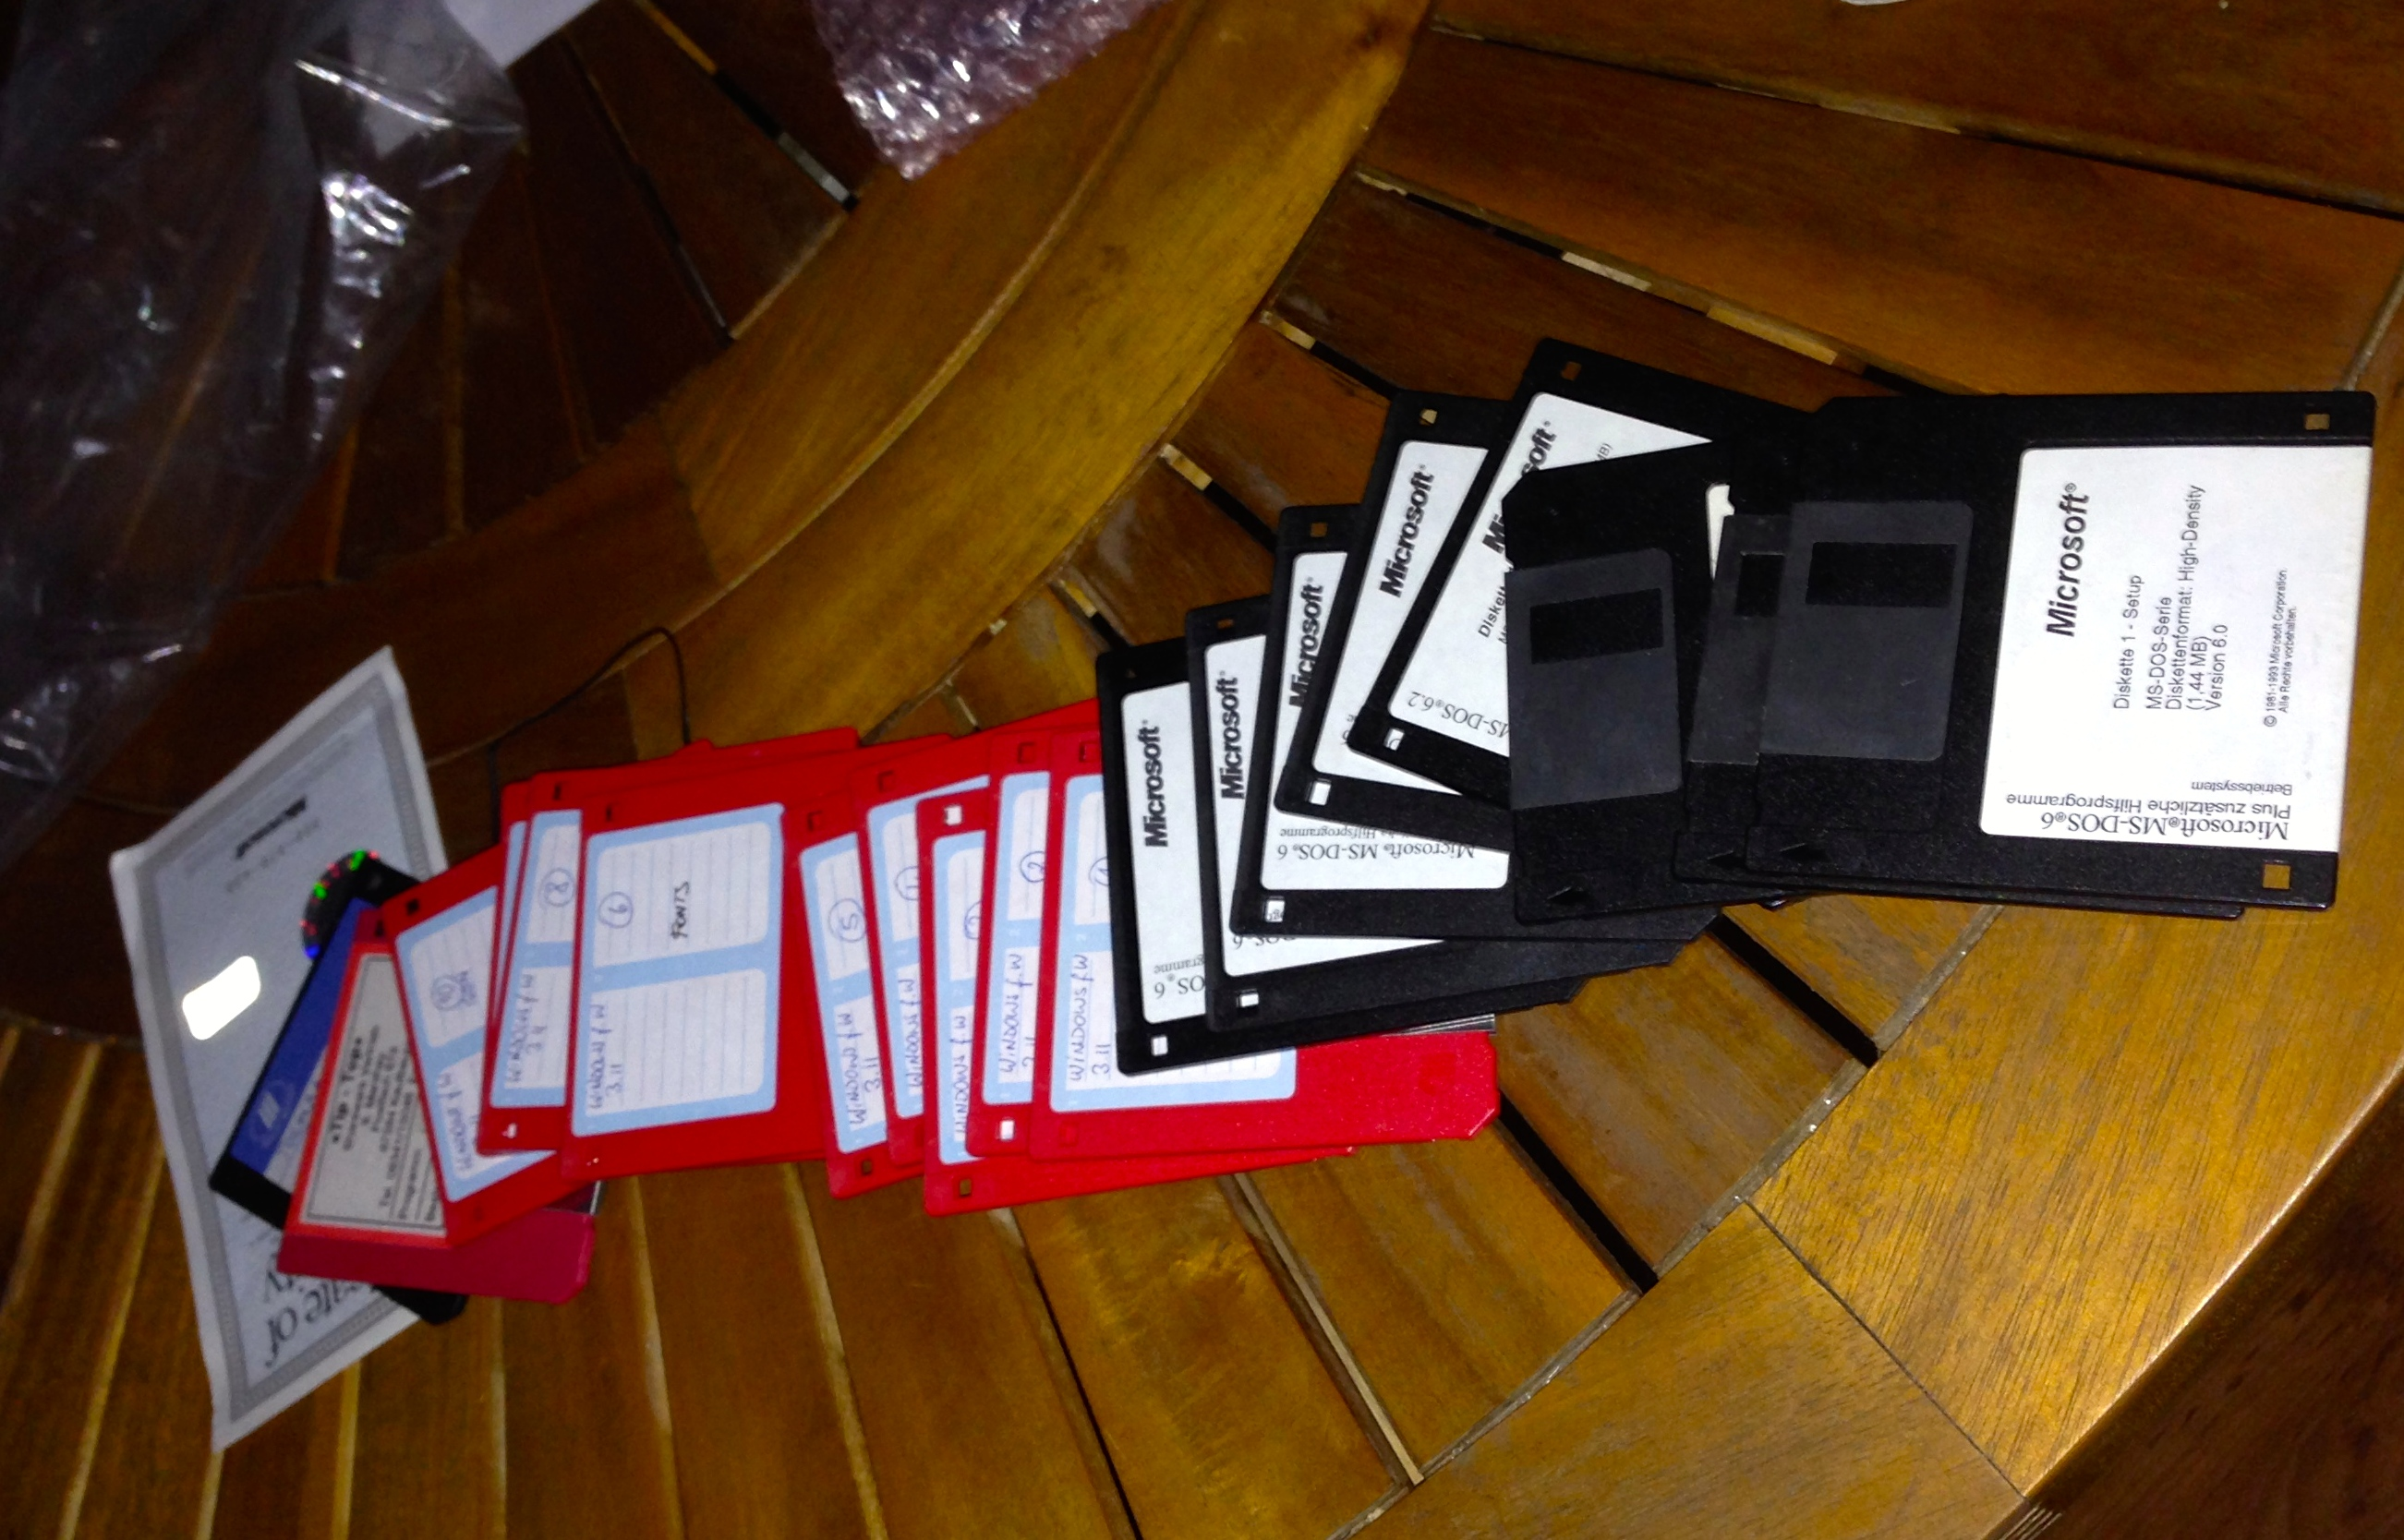
\includegraphics[width=0.8\textwidth]{img/win311disks.jpg}
			\caption{Windows 3.11 und MS DOS 6.22 auf Disketten}
			\label{fig:screenshot-win311disks}
		\end{center}
	\end{figure}

	Stellt man VMWare in den Kompatibilitätseinstellungen auf Version 8 des Hypervisors um, kennt es einen Modus für Windows 3.11, in dem sich das Betriebssystem problemlos von den Diskettenimages installieren lässt. Leider gibt es keine VMWare Guest Additions für dieses Betriebssystem und somit funktionieren nach Installation weder Sound, Netzwerk noch CDROM\footnote{Die in diesem Kapitel installierten Treiber wurden alle von \cite{VMDriver} geladen}.

	Da sowohl MS DOS als auch Windows vor Version 95 im Leerlauf busy waiting statt dem $HLT$-Befehl verwenden, ist die CPU der virtuellen Maschine zudem immer vollständig ausgelastet.
	Dies ist besonders auf einem zentralen Cloud-System, bei dem viele virtuelle Maschinen parallel ausgeführt werden sollen, sehr störend, da jede VM die ihr zur Verfügung stehenden Ressourcen somit voll belegt, auch wenn sie nicht benutzt werden.
	Eine Lösung findet sich auf \cite{VMDriver} mit dem Programm "`CPUidle for DOS"' von Marton Balog.
	Bei diesem handelt es sich um eine TSR, die das busy waiting von MS DOS überschreibt, statt dessen die CPU in dieser Zeit anhält und durch Interrupts wieder aufweckt.
	Gleiches bewirkt unter Windows 3.11 der Treiber "`WQGHLT"' aus der selben Quelle.

	\begin{figure}[h]
		\begin{center}
			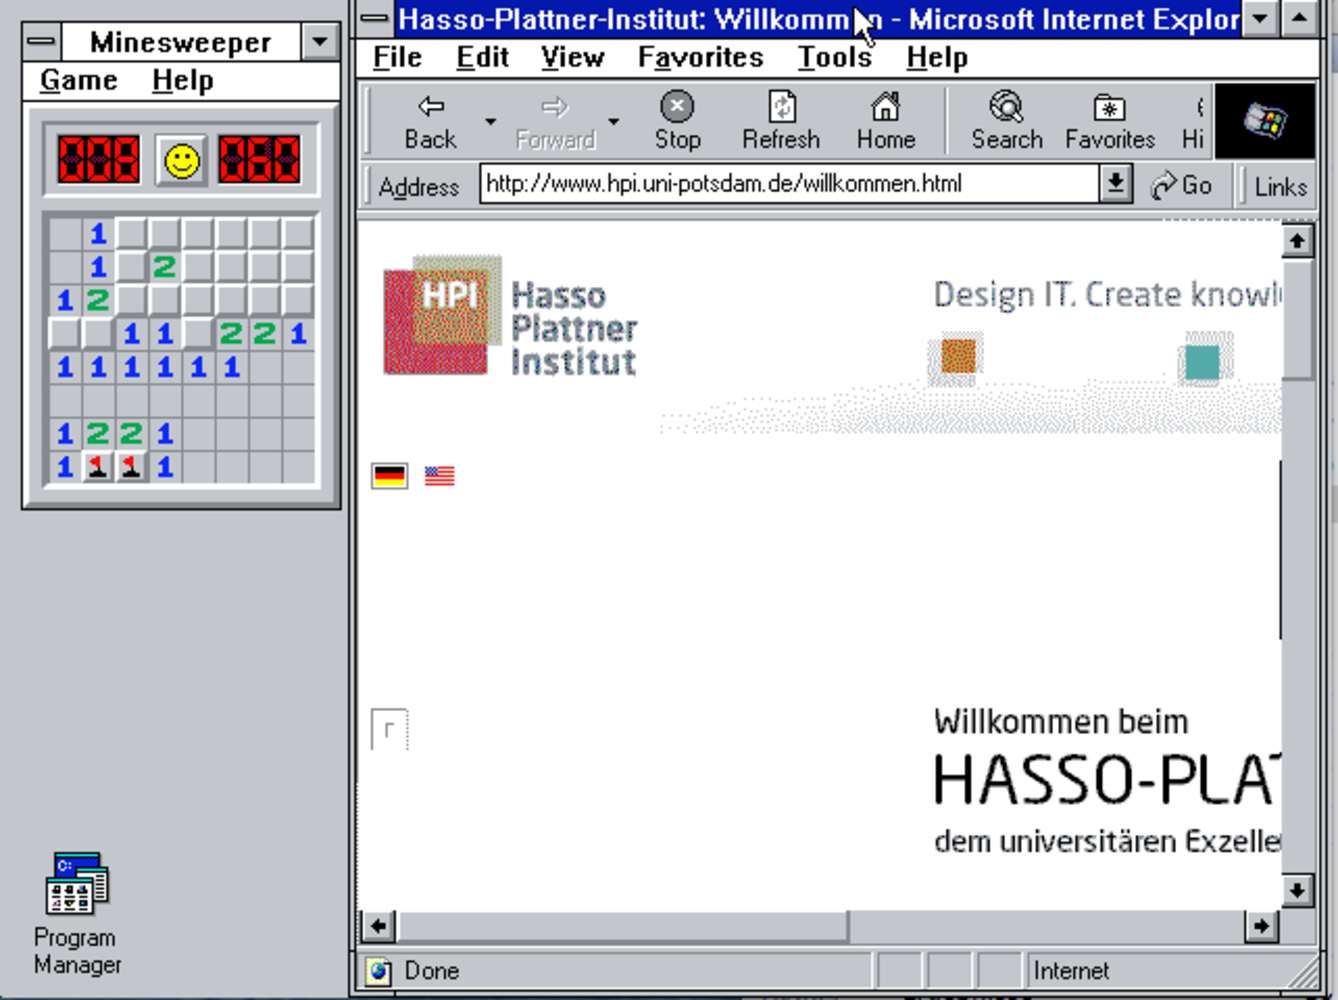
\includegraphics[width=\textwidth]{img/win311screen}
			\caption{Windows 3.11 mit Minesweeper und Internet Explorer 5.0}
			\label{fig:screenshot-win311apps}
		\end{center}
	\end{figure}

	Die Netzwerkfunktionalität kann aktiviert werden, indem der Treiber für die "`Advanced Micro Devices PCNET Family"' nachinstalliert wird.
	Zudem muss explizit der TCP/IP-Protokolltreiber installiert werden, da Windows 3.11 standardmäßig nur die veralteteten Protokollen IPX/SPX und NetBEUI unterstützt.

	Leider nicht mehr aktivieren lässt sich die Unterstützung für Audioausgabe, da VMWare die Karte SoundBlaster16 nur bis zur Version 5 emuliert.
	Neuere Hypervisoren emulieren leistungsfährigere Soundkarten, für die es aber keine Treiber mehr für Windows 3.11 gibt.


	Bei WinWorld finden sich außerdem auf diesem Betriebssystem lauffähige Versionen von Internet Explorer und Netscape Navigator.
	Letzterer stürzt aufgrund eines Bugs jedoch im Hypervisor und auf neueren CPUs als Pentium ab, dabei bringt er Windows komplett zum Absturz und ist ein gutes Beispiel für den fehlenden Speicherschutz.

	Der Internet Explorer lässt sich hingegen in Version 5.0 installieren und ausführen. 
	Hiermit lässt sich ansatzweise im Internet surfen, jedoch werden nahezu alle Webseiten werden fehlerhaft dargestellt, da noch kein CSS der Version 2 unterstützt wird und außerdem nur Seiten bis zu einer Größe von 1 MB verarbeitet werden können. \\



%%%%%%%%%%%%%%%%%%%%%%%%%%%%%%%%%%%%%%%%%%%%%%%%%%%%%%%%%%%%%%%%%%%%%%%%%%%%%%%%%%%%%%%%%%%%%%%%%%%%%%%%%
\section{Windows NT 3.51}
%%%%%%%%%%%%%%%%%%%%%%%%%%%%%%%%%%%%%%%%%%%%%%%%%%%%%%%%%%%%%%%%%%%%%%%%%%%%%%%%%%%%%%%%%%%%%%%%%%%%%%%%%

	Als besonders schwierig gestaltete sich die Installation von Windows NT 3.51. 
	Standardmäßig wird dieses System von VMWare nicht unterstützt und ist durch einen Bug im Memory Management nicht lauffähig\footnote{\url{http://kb.vmware.com/selfservice/microsites/search.do?language=en_US&cmd=displayKC&externalId=1021509}}.
	Im Internet finden sich jedoch ein paar Tricks, mit denen der Betrieb des Systems gelingt\footnote{\url{http://www.lo-tech.co.uk/wiki/Installing_Windows_NT_3.51_on_VMware}}.

	\begin{figure}[h]
		\begin{center}
			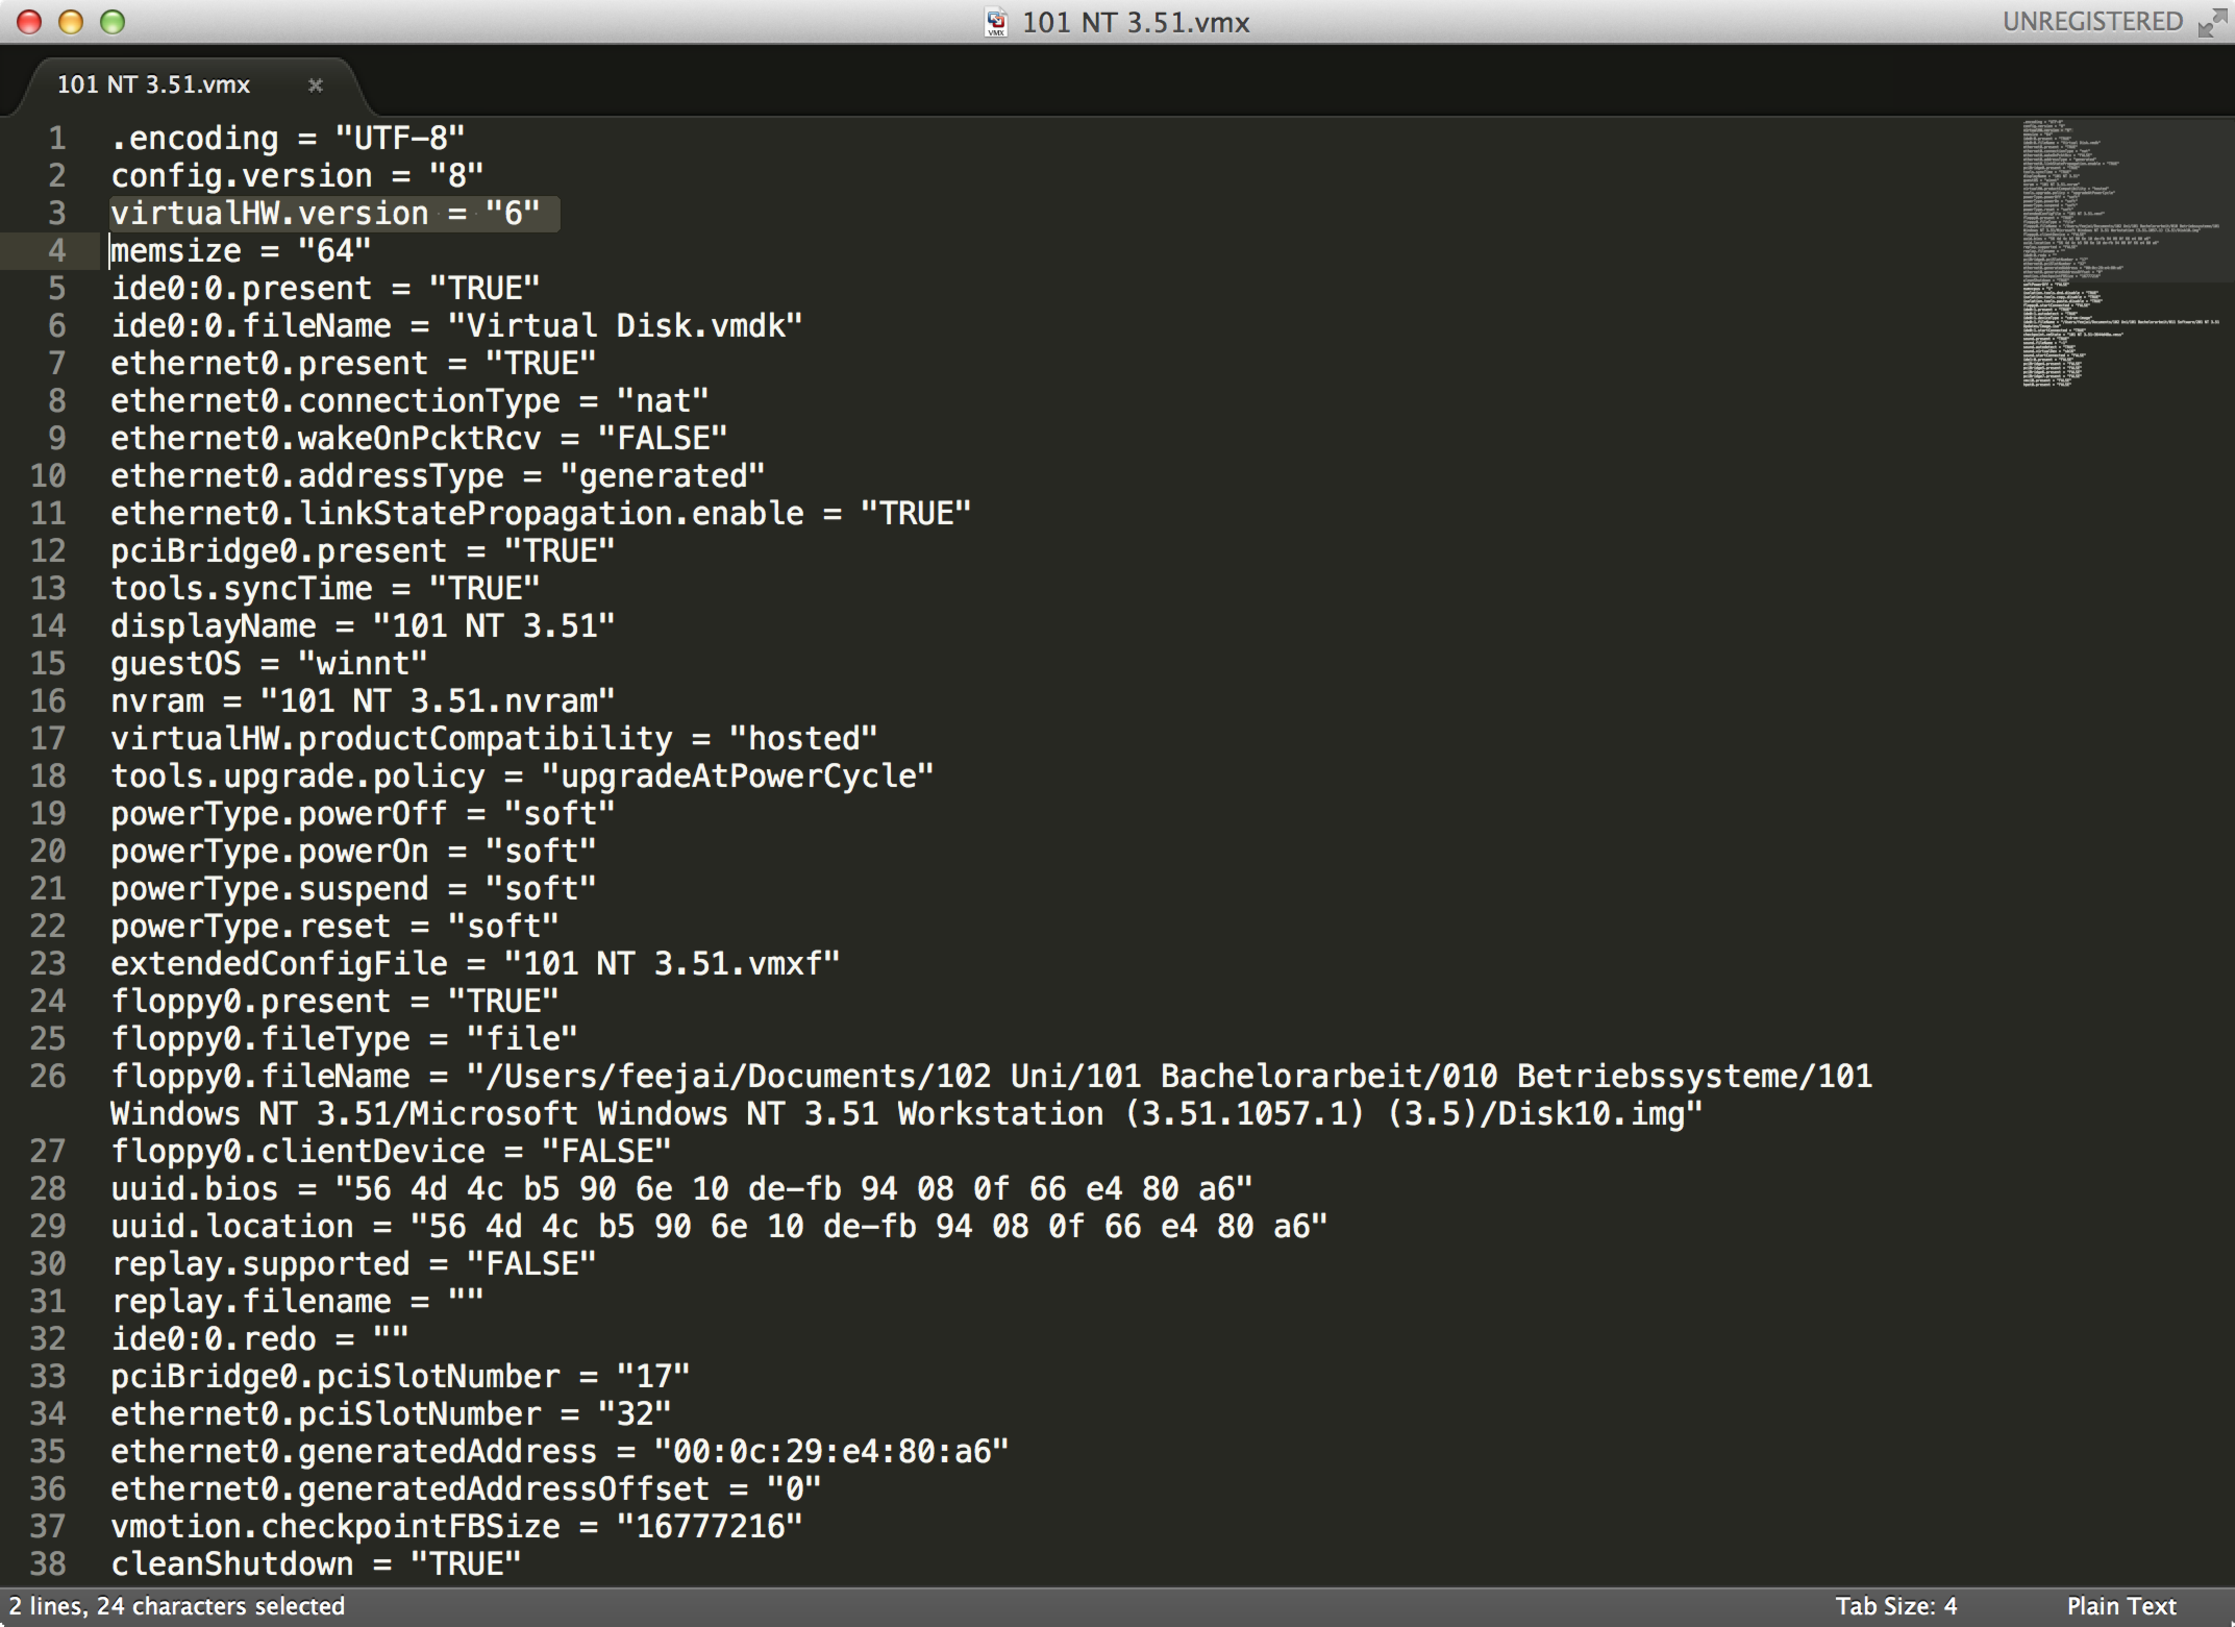
\includegraphics[width=0.8\textwidth]{img/351vmx}
			\caption{Hypervisorkonfiguration für NT 3.51}
			\label{fig:screenshot-351vmx}
		\end{center}
	\end{figure}

	Zunächst muss beim Anlegen der virtuellen Maschine darauf geachtet werden beim Betriebssystem als Typ 'other' und nicht 'Windows NT' zu wählen.
	Vor der Start muss außerdem die .vmx-Datei in einem Texteditor geöffnet und die folgenden Änderungen durchgeführt werden:

		\begin{itemize}
			\item Die Version des Hypervisors muss auf 6 geändert werden: \\ \texttt{virtualHW.version = \string"6\string"}
			\item Die Zeile \texttt{vmci0.present = \string"TRUE\string"}
			\item Sämtliche Zeilen \texttt{pciBridge?.present = \string"TRUE\string"} müssen entfernt werden.
		\end{itemize}


	Die Installation von CD funktionierte nicht in VMWare, daher musste die Installation mit den ebenfalls möglichen Bundle aus 22 Disketten durchgeführt werden. 

	Nach der Installation muss das Betriebssystem im Hypervisor wieder zurück auf 'Windows NT' geändert werden. 
	Anschließend lässt sich das System benutzen, es existieren jedoch keine Netzwerk oder Soundtreiber.


%%%%%%%%%%%%%%%%%%%%%%%%%%%%%%%%%%%%%%%%%%%%%%%%%%%%%%%%%%%%%%%%%%%%%%%%%%%%%%%%%%%%%%%%%%%%%%%%%%%%%%%%%
\section{Windows NT 4.0 SP 6}
%%%%%%%%%%%%%%%%%%%%%%%%%%%%%%%%%%%%%%%%%%%%%%%%%%%%%%%%%%%%%%%%%%%%%%%%%%%%%%%%%%%%%%%%%%%%%%%%%%%%%%%%%

	Windows NT 4 wird von VMWare unterstützt. 
	Hierbei muss bei der Installation "`Windows NT"' als Betriebssystemtyp gewählt und eine virtuelle SCSI-Festplatte angelegt werden. 
	
		\begin{figure}[h]
		\begin{center}
			\includegraphics[width=\textwidth]{img/nt4}
			\caption{Windows NT 4 mit HPI-Homepage}
			\label{fig:screenshot-nt4}
		\end{center}
	\end{figure}


	Nach Installation des Service Packs 6a lässt sich der Internet Explorer 6 installieren.
	Damit ist Netzwerkzugriff möglich. 
	Von Microsoft wird ebenfalls ein Post-SP6a Hotfixpaket angeboten\footnote{\url{http://support.microsoft.com/kb/299444/de}}, das ebenfalls installiert werden muss, damit die die VMWare Guest Additions funktionieren.


	Nach der Installation der Guest Additions läuft das System stabil und zuverlässig. 

	Um die Updates durchzuführen, wurden die notwendigen Dateien zunächst auf dem Hostsystem heruntergeladen und auf ein ISO-Image kopiert. Dies wurde in VMWares virtuelles CD-Laufwerk geladen und von dort die Installation durchgeführt.

%%%%%%%%%%%%%%%%%%%%%%%%%%%%%%%%%%%%%%%%%%%%%%%%%%%%%%%%%%%%%%%%%%%%%%%%%%%%%%%%%%%%%%%%%%%%%%%%%%%%%%%%%
\section{Windows 2000 Professional}
%%%%%%%%%%%%%%%%%%%%%%%%%%%%%%%%%%%%%%%%%%%%%%%%%%%%%%%%%%%%%%%%%%%%%%%%%%%%%%%%%%%%%%%%%%%%%%%%%%%%%%%%%

	Die mitgeliegerte Windows 2000 VM wurde mit einem Datenträger von Maniac, dem Softwareportal für HPI-Studenten, installiert.

	Windows 2000 wird von VMware vollständig unterstützt, alle notwendigen Treiber werden über die Guest Additions installiert und die Service Packs können von Microsoft herunter geladen werden.
	Auf die Installation wird daher an dieser Stelle nicht gesondert eingegangen.



%%%%%%%%%%%%%%%%%%%%%%%%%%%%%%%%%%%%%%%%%%%%%%%%%%%%%%%%%%%%%%%%%%%%%%%%%%%%%%%%%%%%%%%%%%%%%%%%%%%%%%%%%
\section{Konvertierung in KVM und Integration ins InstantLab}
%%%%%%%%%%%%%%%%%%%%%%%%%%%%%%%%%%%%%%%%%%%%%%%%%%%%%%%%%%%%%%%%%%%%%%%%%%%%%%%%%%%%%%%%%%%%%%%%%%%%%%%%%

	Obwohl durch OpenStack verschiedene Hypervisoren, wie KVM, VMWare und Hyper-V unterstützt werden\footnote{\url{https://wiki.openstack.org/wiki/HypervisorSupportMatrix}},
	verwendet das InstantLab zum gegenwärtigen Zeitpunkt lediglich KVM Execution Hosts.
	Aus diesem Grunde sollten die erzeugen VMWare-Images zu QEMU/KVM im Rahmen dieser Arbeit konvertiert werden.
	Hierbei wurde nach Anleitung in \cite{VMVDiskMan} vorgegangen. 
	Leider war die Konversion bestehender Images nicht erfolgreich und außer Windows 2000 ließ sich kein System booten.

	Daher wurden vom Autor ein Ubuntu Linux 13.10 installiert, in dem mittels QEMU versucht wurde, die Virtuellen Maschinen erneut zu erstellen.
	Die offizielle Dokumentation des "`Guest Support Status"' von KVM geht nur zurück bis Windows 95;
	der Status lautet: "`no way!"' \cite{KVMStatus}.

	Leider entsprachen die im Experiment gesammelten praktischen Erfahrungen relativ genau denen der durch die Dokumentation zu erwartenden:
	\begin{itemize}
		\item \emph{DOS 5.0} ist funktionsfähig bis 1 MB Arbeitsspeicher. Windows 2.11 kann ohne Maus gestartet werden.
		\item \emph{DOS 6.22} läuft, stürzt aber ab, sobald mittels $himem.sys$ oder $emm386$ der erweiterten Speicher adressiert werden soll. Dies macht den Betrieb von Windows 3.11 unmöglich.
		\item \emph{Windows NT 3.51} lässt sich nicht installieren, das Setup-Programm stürzt ab
		\item \emph{Windows NT 4 SP6} läuft, allerdings existiert weder ein funktionsfähiger Maus-, noch ein Netzwerktreiber
		\item \emph{Windows NT 2000 Professional} ist als einziges vollkommen funktionsfähig
	\end{itemize}


	Für diese Arbeit wurde versucht, die Guest-Additions von KVM für Windows 2000 auf Windows NT 3.51 zu portieren und den Grund für den Absturz zu debuggen.
	Mangels heute verfügbarer Dokumentantion zur Treiberentwicklung unter diesem System, unzureichender technischer Dokumentation von KVM und weiter Teile des Linux Kernels und zu geringer Kenntnisse über die Funktionsweise von Hypervisoren waren diese Versuche nicht erfolgreich und wurden bald aufgegeben. 

	Stattdessen wurde von Andreas Grapentin, dem Administrator des InstantLabs, vorgeschlagen, InstantLab zusätzlich mit VMWare Hypervisoren auszustatteten.
	OpenNebula, die verwendete OpenStack Implementierung, ermöglicht neben KVM und VirtualBox die Anbindung von verschiedenen VMWare Produkten als Execution Hosts.
	Die Wahl fällt hier auf den VMWare ESXi, eine kostenfreie Implementierung des VMWare ESX Servers als "`bare-metal Hypervisor"'. 

	KVM wird daher in dieser Arbeit nicht weiter verfolgt, statt dessen wurden alle Virtuellen Maschinen auf Kompatibilität mit dem VMWare ESXi geprüft.


		%%% %%%%%%%%%%%%%%%%%%%%%%%%%%%% %%%
%%% Main Chapter 2 : Challenges  %%%
%%% %%%%%%%%%%%%%%%%%%%%%%%%%%%% %%%
\chapter{Experimente}
\label{chap:experiments}

In diesem Kapitel werden die einzelnen Experimente beschrieben, mit denen einige Neuerungen und auch Probleme der jeweiligen Version getestet werden können. Es soll später als Experimentierhandbuch verwendet werden können.

Jeder Abschnitt beschreibt zunächst die notwendigen Vorbereitungen.
Anschließgend folgt eine Serie von Handlungsanweisungen.
Schließlich folgt eine Erklärung des erwarteten Verhalten und Möglichkeiten diese zu Beobachten.


%Was tun?
%Was beobachten?
%Aufbau?
%erwartetes Verhalten?

%Bspw. Übung: TSR durch Memory Abbild

%%%%%%%%%%%%%%%%%%%%%%%%%%%%%%%%%%%%%%%%%%%%%%%%%%%%%%%%%%%%%%%%%%%%%%%%%%%%%%%%%%%%%%%%%%%%%%%%%%%%%%%%%
\section{DOS 5.0}
%%%%%%%%%%%%%%%%%%%%%%%%%%%%%%%%%%%%%%%%%%%%%%%%%%%%%%%%%%%%%%%%%%%%%%%%%%%%%%%%%%%%%%%%%%%%%%%%%%%%%%%%%


	\subsection{TSR}

	Unter MS DOS konnten noch keine Anwendungen parallel ausgeführt werden. Insbesondere waren  Daemons oder Backgroundprozesse nicht vorgesehen.
	Um zu kleinen Tools wie bspw. einem Taschenrechner wechseln zu können, ohne die eigentliche Anwendung beenden zu müssen, konnte man sich mit sogenannten TSRs, "`Teminate and Stay Resident"'-Programmen behelfen\footnote{Eine hervorragende Einführung in die Programmierung und die Funktionsweise von TSRs befindet sich unter: \url{https://courses.engr.illinois.edu/ece390/books/artofasm/CH18/CH18-1.html\#HEADING1-3}}.
	%Ebenso waren die meisten Computerviren zu dieser Zeit TSRs. 

	\begin{figure}[h]
		\begin{center}
			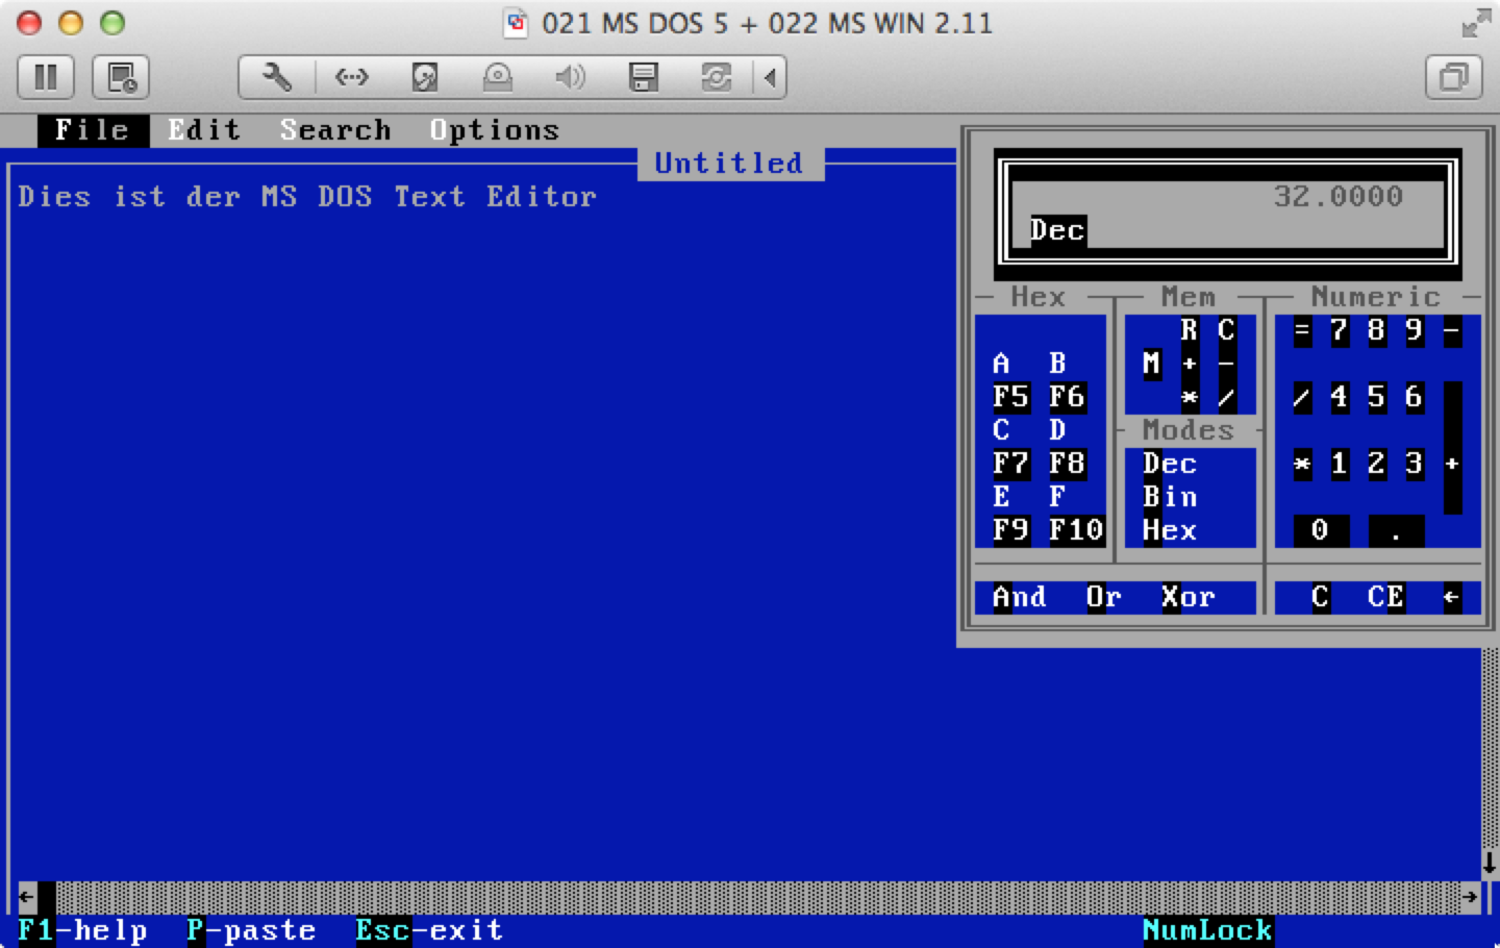
\includegraphics[width=0.8\textwidth]{img/dostsr}
			\caption{TSR-Taschenrechner vor dem DOS-Editor}
			\label{fig:screenshot-dostsr}
		\end{center}
	\end{figure}

	Eine sehr beliebte TSR war Borland Sidekick, die unter anderm einen Notizzettel, einen Taschenrechner und einen Kalender bereitstellte. Mit dem Befehl ctrl+alt konnte man diese jederzeit aufrufen.

	Machen Sie sich nun mit der Funktionsweise dieser TSR vertraut:
	
		\begin{itemize}
			\item Starten Sie die VM und beenden Sie die DOS Shell. Notieren Sie zunächst den freien Speicher, der mit dem Befehl \texttt{mem} ausgegeben werden kann.
			\item Starten Sie Sidekick (\texttt{$C:\backslash{}sk\backslash{}sk.com$}). Dieses Programm beendet sich sofort wieder. Überprüfen Sie erneut den freien Speicher. Wodurch kommt die Veränderung zustande?
			\item Starten Sie ein anderes Programm, zum Beispiel den Standard DOS Texteditor \texttt{EDIT}. Testen Sie dabei die Verwendung der Funktionen von Sidekick. Wodurch gelingt es Sidekick, wieder in den Vordergrund zu treten, obwohl die CPU an eine andere Anwendung abgegeben wurde?
			\item Was passiert bei der Verwendung einer TSR unter Windows?
		\end{itemize}
	  

	\subsection{Busy Waiting}

	Obwohl seit dem 8088er vorhanden, benutzt MS DOS noch nicht die \texttt{HLT}-Instruction der x86 CPU.
	
	\begin{itemize}
		\item Starten Sie die MS DOS VM und beobachten Sie ihr Verhalten. Beenden Sie hierzu die DOS Shell
		\item Wie viel CPU und wie viel RAM verbraucht die VM? Wie verändern sich diese Parameter unter Last? Wie verhält sich MS DOS folglich im Leerlauf?
		\item Starten Sie nun die Anwendung \texttt{DOSIDLE}. Um was für eine Anwendung handelt es sich?
		\item Wie hat sich die Ressourcennutzung der VM durch den Start der Anwendung verändert? Wodurch könnte dies erreicht werden?
	\end{itemize}


	\subsection{DOS-Shell}

	MS DOS wird in Version 5 wird mit einer an den Norton Commander angelehnten graphischen Shell ausgeliefert. Diese wird beim Start des Betriebssystems automatisch geladen.

	\begin{itemize}
		\item Machen Sie sich mit der Bedienung der DOS Shell vertraut. Benutzen Sie hierfür die $Alt$-Taste, um in die Menüs zu gelangen.
		\item Wie können aus dieser Shell Anwendungen gestartet werden? Starten und beenden Sie den Basic Interpreter QBasic
		\item Was passiert, wenn eine TSR, z.B. Sidekick aus der DOS Shell gestartet wird? 
	\end{itemize}

%%%%%%%%%%%%%%%%%%%%%%%%%%%%%%%%%%%%%%%%%%%%%%%%%%%%%%%%%%%%%%%%%%%%%%%%%%%%%%%%%%%%%%%%%%%%%%%%%%%%%%%%%
\section{Windows 2.11}
%%%%%%%%%%%%%%%%%%%%%%%%%%%%%%%%%%%%%%%%%%%%%%%%%%%%%%%%%%%%%%%%%%%%%%%%%%%%%%%%%%%%%%%%%%%%%%%%%%%%%%%%%

	\subsection{Koop. Multitasking}

	Anders als unter MS DOS können unter Windows mehrere Anwendungen gleichzeitig ausgeführt werden. 
	Dadurch ist die Verwendung von TSRs nicht mehr notwendig.

	\begin{itemize}
		\item Starten Sie Microsoft Windows 2.11 und machen Sie sich mit den mitgelieferten Applikationen vertraut.
		\item Starten Sie Microsoft Excel und eine weitere Anwendung. Wie ist Copy \& Paste implementiert?
		\item Was passiert beim Absturz einer Anwendung? Warum?
	\end{itemize}


%%%%%%%%%%%%%%%%%%%%%%%%%%%%%%%%%%%%%%%%%%%%%%%%%%%%%%%%%%%%%%%%%%%%%%%%%%%%%%%%%%%%%%%%%%%%%%%%%%%%%%%%%
\section{DOS 6.22}
%%%%%%%%%%%%%%%%%%%%%%%%%%%%%%%%%%%%%%%%%%%%%%%%%%%%%%%%%%%%%%%%%%%%%%%%%%%%%%%%%%%%%%%%%%%%%%%%%%%%%%%%%

	\subsection{Extended Memory}

	MS DOS verwendet den Real Mode der x86 CPU, indem diese aufgrund der Registerbreite maximal 1 MiB RAM adressieren kann. Davon stellt MS DOS bis zu 640kiB Anwendungen zur Verfügung. Ende der 80er war dies jedoch für die meisten Programme bereits deutlich zu wenig.

	\begin{itemize}
		\item Starten Sie Microsoft Windows 2.11 und machen Sie sich mit den mitgelieferten Applikationen vertraut.
		\item Starten Sie Microsoft Excel und eine weitere Anwendung. Wie ist Copy \& Paste implementiert?
		\item Was passiert beim Absturz einer Anwendung? Warum?
	\end{itemize}

	\subsection{DoubleSpace oder DriveSpace}

	Ein häufiges Problem zur Zeit von MS DOS war der begrenze Speicherplatz. Mit MS DOS 6.0 wurde daher die Datenträgerkomprimierung DoubleSpace eingeführt.
	Diese musste aus patentrechtlichen Gründen jedoch von Microsoft bald wieder entfernt werden und wurde mit DOS 6.22 durch DriveSpace, ein Programm mit ähnlicher Funktionsweise aber anderem Kompressionsalgorithmus ersetzt.

	\begin{itemize}
		\item Starten Sie die VM und legen Sie das mitgelieferte, leere 1,44MB-Diskettenimage in Laufwerk A: ein.
		\item Erzeugen Sie mit dem Befehl Type eine Textdatei mit einer Größe von mindestens 1,5 MB.
		Was passiert, wenn Sie versuchen, diese auf Volume A: zu kopieren?
		\item Legen Sie mittels DriveSpace ein komprimiertes Dateisystem auf diesem Image an. Lesen Sie hierfür ggf. $help drvspace$.
		\item Versuchen Sie erneut, die Textdatei auf Volume A: zu kopieren. 
		\item Wie unterscheiden sich die Werte des $Volume$ und der $dir$-Kommandos?
	\end{itemize}

%%%%%%%%%%%%%%%%%%%%%%%%%%%%%%%%%%%%%%%%%%%%%%%%%%%%%%%%%%%%%%%%%%%%%%%%%%%%%%%%%%%%%%%%%%%%%%%%%%%%%%%%%
\section{Windows 3.11 for Workgroups}
%%%%%%%%%%%%%%%%%%%%%%%%%%%%%%%%%%%%%%%%%%%%%%%%%%%%%%%%%%%%%%%%%%%%%%%%%%%%%%%%%%%%%%%%%%%%%%%%%%%%%%%%%

	\subsection{Netzwerk}

		Windows 3.11 ermöglicht erstmals Datei- und Printersharing über das SMB-Protokoll.
	
		\begin{itemize}
			\item Legen Sie zunächst eine Heimnetzgruppe auf mindestens zwei virtuellen Maschinen an.
			\item Kopieren Sie eine Datei von ihrem Übungspartner.
		\end{itemize}

	\subsection{Internetzugriff}

		Ebenfalls ab Windows 3.11 ist der Zugriff auf das Internet möglich.
		Hierfür wurde das TCP/IP-Protokoll nachgerüstet. 

		\begin{itemize}
			\item Starten Sie den vorinstallierten Internet Explorer 5.
			\item Rufen Sie nun einige Webseiten auf und vergleichen Sie, wie sehr sich das Internet in den letzten 20 Jahren gewandelt hat. Können Sie ein aktuelle Webseite finden, die fehlerfrei dargestellt wird?
			\item Ebenfalls installiert ist der Netscape Navigator 4.
		Dieser ist auf neuen CPUs durch einen Bug nicht lauffähig und stürzt beim Start ab. 
		Warum stürzt hierbei das gesamte Betriebssystem ab?
		\end{itemize}

%%%%%%%%%%%%%%%%%%%%%%%%%%%%%%%%%%%%%%%%%%%%%%%%%%%%%%%%%%%%%%%%%%%%%%%%%%%%%%%%%%%%%%%%%%%%%%%%%%%%%%%%%
\section{Windows NT 3.51}
%%%%%%%%%%%%%%%%%%%%%%%%%%%%%%%%%%%%%%%%%%%%%%%%%%%%%%%%%%%%%%%%%%%%%%%%%%%%%%%%%%%%%%%%%%%%%%%%%%%%%%%%%

	\subsection{NTFS}

	Windows NT 3.51 wird mit dem neuartigen Dateisystem NTFS ausgeliefert. Hierbei besteht jede Datei aus beliebig vielen Datenströmen ("`Streams"'').
	Außerdem kann eine Datei mehreren Namen, insbesondere einen 8+3-Kurznamen besitzen. 

	\begin{itemize}
		\item Starten Sie die Eingabeaufforderung über Main > Command Prompt
		\item Erstellen Sie einen neuen Ordner und legen Sie die Textdatei uebung.txt an.
		Speichern Sie hierbei den Text 'dcl' in den alternativen Stream 'alternativ.txt'\\
		\texttt{echo \string"dcl\string" > uebung.txt:alternativ.txt}
		\item Wie groß ist diese Textdatei laut Befehl \texttt{dir} und im Windows Explorer?
		\item Editieren Sie die Textdatei in Notepad. Wieso ist diese Datei leer? 
		\item Geben Sie einen Text ein. Wohin werden Daten gespeichert? Wie groß ist die Datei jetzt?
		\item Öffnen Sie nun den alternativen Stream und führen Sie einige Änderungen durch: \\
			\texttt{notepad uebung.txt:alternativ.txt}
	\end{itemize}

	\subsection{VGA im User Mode}

	In Windows NT der 3. Generation wird die Grafik (GDI) vom Client-Server Runtime Subsystem im User-Mode erzeugt.
	Was passiert, wenn Sie CSRSS im Task-Manager beenden?

%%%%%%%%%%%%%%%%%%%%%%%%%%%%%%%%%%%%%%%%%%%%%%%%%%%%%%%%%%%%%%%%%%%%%%%%%%%%%%%%%%%%%%%%%%%%%%%%%%%%%%%%%
\section{Windows NT 4.0 SP 6}
%%%%%%%%%%%%%%%%%%%%%%%%%%%%%%%%%%%%%%%%%%%%%%%%%%%%%%%%%%%%%%%%%%%%%%%%%%%%%%%%%%%%%%%%%%%%%%%%%%%%%%%%%

	\subsection{CSRSS}

	Mit Windows NS wurde GDI vom CSRSS in den Kernelmode verschoben.
	Die Ausgabe auf der Kommandozeile wird jedoch nach wie vor durch das CSRSS erledigt. 
	Dieses ist ein Systemprozess im User-Mode, der standardmäßig mit der Schedulingpriorität 24 läuft.

	Für dieses Experiment wurden zwei Executables erzeugt:
		\begin{enumerate}
			\item \emph{Experiment1.exe} ist eine CLI-Applikation die zweimal pro Sekunde einen Punkt auf die Kommandozeile schreibt, bis man sie beendet.
			\item \emph{Experiment2.exe} lastet nach Anforderung die CPU für ca. 10 Sekunden mit einer Zählschleife aus.
		\end{enumerate}

	\begin{itemize}
		\item Starten Sie Experiment1.exe und Experiment2.exe. 
		\item Stellen Sie im Task-Manager die Prioritätsklasse 'Echtzeit' für beide Prozesse ein. Die Prozesse setzen die Priorität ihrer Threads auf \texttt{$THREAD\_PRIORITY\_HIGHEST$}, sodass diese insgesamt mit einer Schedulingpriorität von 26 laufen\footnote{\url{http://msdn.microsoft.com/en-us/library/windows/desktop/ms685100(v=vs.85).aspx}}.
		\item Blockieren Sie nun die CPU mit Experiment2.exe. Obwohl beide Prozesse die gleiche Priorität haben, werden von Experiment1.exe keine Punkte mehr ausgegeben. Wieso?
	\end{itemize}


	\emph{Lösung:} Der Scheduler teilt beiden Prozessen wie erwartet die gleiche Rechenzeit zu.
	Experiment1.exe übergibt die Ausgabe an das CSRSS und blockiert, bis diese durchgeführt wurde.
	Da das CSRSS mit einer niedrigeren Priorität als Experiment2.exe läuft, wird dieses jedoch verdrängt.
	Folglich erhält Experiment1.exe keine Rechenzeit mehr, bis die CPU von Experiment2.exe wieder freigegeben wird und das CSRSS aufgerufen wurde.

	%\subsection{EXEType}

%%%%%%%%%%%%%%%%%%%%%%%%%%%%%%%%%%%%%%%%%%%%%%%%%%%%%%%%%%%%%%%%%%%%%%%%%%%%%%%%%%%%%%%%%%%%%%%%%%%%%%%%%
\section{Windows 2000 Professional}
%%%%%%%%%%%%%%%%%%%%%%%%%%%%%%%%%%%%%%%%%%%%%%%%%%%%%%%%%%%%%%%%%%%%%%%%%%%%%%%%%%%%%%%%%%%%%%%%%%%%%%%%%

	%\subsection{Active Directory}

	\subsection{EFS}

	Windows 2000 erlaubt die Verschlüsselung von Dateien, so dass diese selbst bei Versagen der ACLs vor unauthorisiertem Zugriff geschützt sind.

	\begin{itemize}
		\item Schützen Sie den Administratoraccount mit einem Kenntwort 
		\item Legen Sie eine Textdatei im Ordner 'Eigene Dateien' an.
		\item Wählen Sie die Option 'Inhalt verschlüsseln, um Daten zu schützen' in den Eigenschaften.
		\item Legen Sie einen zweiten Useraccount mit Administratorrechten an.
		\item Was passiert, wenn Sie von diesem Account auf die Datei zugreifen wollen?
	\end{itemize}


		%%% %%%%%%%%%%%%%%%%%%%%%%%%%%%% %%%
%%% Main Chapter 5 : Evaluation  %%%
%%% %%%%%%%%%%%%%%%%%%%%%%%%%%%% %%%
\chapter{Fazit}
\label{chap:evaluation}


%%%%%%%%%%%%%%%%%%%%%%%%%%%%%%%%%%%%%%%%%%%%%%%%%%%%%%%%%%%%%%%%%%%%%%%%%%%%%%%%%%%%%%%%%%%%%%%%%%%%%%%%%
\section{Ergebnisse}
\label{sec:results}
%%%%%%%%%%%%%%%%%%%%%%%%%%%%%%%%%%%%%%%%%%%%%%%%%%%%%%%%%%%%%%%%%%%%%%%%%%%%%%%%%%%%%%%%%%%%%%%%%%%%%%%%%



		
		

%%%%%%%%%%%%%%%%%%%%%%%%%%%%%%%%%%%%%%%%%%%%%%%%%%%%%%%%%%%%%%%%%%%%%%%%%%%%%%%%%%%%%%%%%%%%%%%%%%%%%%%%%
\section{Zukünftige Erweiterungen}
\label{sec:future}
%%%%%%%%%%%%%%%%%%%%%%%%%%%%%%%%%%%%%%%%%%%%%%%%%%%%%%%%%%%%%%%%%%%%%%%%%%%%%%%%%%%%%%%%%%%%%%%%%%%%%%%%%

		%%%%%%%%%%%%%%%%%%%%%%%%%%%%%%%%%%%%%%%%%%%%%%%%%%%%%%%%%%%%
		\subsection{Weitere Betriebssysteme}
		%%%%%%%%%%%%%%%%%%%%%%%%%%%%%%%%%%%%%%%%%%%%%%%%%%%%%%%%%%%%
	
		%%%%%%%%%%%%%%%%%%%%%%%%%%%%%%%%%%%%%%%%%%%%%%%%%%%%%%%%%%%%
		\subsection{Experimente zu anderen Neuerungen}
		%%%%%%%%%%%%%%%%%%%%%%%%%%%%%%%%%%%%%%%%%%%%%%%%%%%%%%%%%%%%		
		
		Killer-Features meist mehr als 1				
		

		%%%%%%%%%%%%%%%%%%%%%%%%%%%%%%%%%%%%%%%%%%%%%%%%%%%%%%%%%%%%
		\subsection{Didaktische Verbesserungen}
		%%%%%%%%%%%%%%%%%%%%%%%%%%%%%%%%%%%%%%%%%%%%%%%%%%%%%%%%%%%%


%%%%%%%%%%%%%%%%%%%%%%%%%%%%%%%%%%%%%%%%%%%%%%%%%%%%%%%%%%%%%%%%%%%%%%%%%%%%%%%%%%%%%%%%%%%%%%%%%%%%%%%%%
\section{Fazit}
\label{sec:evaluation}
%%%%%%%%%%%%%%%%%%%%%%%%%%%%%%%%%%%%%%%%%%%%%%%%%%%%%%%%%%%%%%%%%%%%%%%%%%%%%%%%%%%%%%%%%%%%%%%%%%%%%%%%%
	
		\printbibliography[heading=bibnumbered]

		%%% %%%%%%%%%%%%%%%%%%% %%%
		%%% Load Appendix Stuff %%%
		%%% %%%%%%%%%%%%%%%%%%% %%%
		%\nocite{*}
		%\bibliography{extra/literatur}
		\appendix
		%%##################################################################################################%
\chapter{Datenbankschema}
\label{chap:schema}
%##################################################################################################%
%##################################################################################################%
%##################################################################################################%


		\lstinputlisting[
						caption=Schema-Beschreibung der vorliegende Umgebungs\-/Informationen im \gls{JSON}-Format. In der Datenbank ebenfalls vorkommende Meta-Informationen wie IDs der Elemente wurden dabei entfernt.,
						language=JavaScript,
						label=lst:sysinfo]
				{src/sysinfo_schema.txt}
		%##################################################################################################%
\chapter{Selbstständigkeitserklärung}
%##################################################################################################%
%##################################################################################################%
%##################################################################################################%

Hiermit bestätige ich, \getauthor, diese Arbeit selbstständig ohne menschliche Hilfe und nur unter Zuhilfenahme der oben aufgeführten Quellen und Hilfsmittel angefertigt zu haben.

\vspace{3cm}

\noindent\getauthor, \getdate

		\printglossary[type=\acronymtype,title=Abkürzungen]
		\listoffigures

\end{document}